%Fiquemos com Deus e Nossa Senhora!
\documentclass[journal]{IEEEtran}

\usepackage{url}
\usepackage{float}
\usepackage{epsfig}
\usepackage{amsmath}
\usepackage{graphicx}
\usepackage{graphics}
\usepackage{setspace}
\usepackage{amssymb}
\usepackage{multirow}
\usepackage{latexsym}
\usepackage{pstricks}
\usepackage{color}
% \usepackage[graphicx]{realboxes}
\usepackage{rotating}


\newcommand{\moldura}[1]{{\fboxsep = 0 pt \framebox{#1}}}

% correct bad hyphenation here
\hyphenation{op-tical net-works semi-conduc-tor}


\begin{document}

\title{FEMa: A Finite Element Machine for Fast Learning}

\author{Danillo~Roberto~Pereira, Marco Ant\^onio Piteri, Andr\'e~Nunes~Souza,        
		Jo\~ao~Paulo~Papa,~\IEEEmembership{Senior,~IEEE,}
        and~Hojjat~Adeli,~\IEEEmembership{Fellow,~IEEE,~Distinguished Member, ~ASCE,~Fellow,~AAAS,~Fellow~AIMBE,~Fellow~American~Neurological~ Association}% <-this % stops a space
\thanks{D. Pereira and J. Papa are with the Department
of Computing, S\~ao Paulo State University, Bauru, SP, 17033-360
 Brazil e-mail: dpereira@ic.unicamp.br, papa@fc.unesp.br}% <-this % stops a space
 \thanks{M. Piteri is with the Department
of Computing, S\~ao Paulo State University, Presidente Prudente, SP
 Brazil e-mail: piteri@fct.unesp.br}
 \thanks{A. Souza is with the Department
of Electrical Engineering, S\~ao Paulo State University, Bauru, SP, 17033-360
 Brazil e-mail: andrejau@feb.unesp.br}
\thanks{H. Adeli is with the Department of Civil, Environmental and Geodetic Engineering, The Ohio State University, Columbus, OH 43210 USA e-mail: adeli.1@osu.edu}% <-this % stops a space
\thanks{This work has been submitted to the IEEE for possible publication.  Copyright may be transferred without notice, after which this version may no longer be accessible.}}

\markboth{Journal of \LaTeX\ Class Files,~Vol.~14, No.~8, August~2015}%
{Shell \MakeLowercase{\textit{et al.}}: Bare Demo of IEEEtran.cls for IEEE Journals}

\maketitle

\begin{abstract}
Machine learning has played an important role in the past decades, being in lockstep with the main advances in computer technology. Given the massive amount of data generated daily, there is a need for even faster and effective learning algorithms that can provide updated models for real-time applications and on-demand tools. In this paper, we propose FEMa - A Finite Element Machine classifier - for supervised learning problems, where each training sample is the center of a basis function, and the whole training set is modeled as a probabilistic manifold for classification purposes. FEMa has its theoretical basis in the Finite Element Method, which is widely used for numeral analysis in engineering problems. We show FEMa is parameterless and it has a quadratic complexity for both training and classification phases when we use basis functions that obey some properties, as well as the proposed classifier can obtain very competitive results when compared against some state-of-the-art supervised pattern recognition techniques.
\end{abstract}

\begin{IEEEkeywords}
Finite element methods, Pattern classification, Pattern recognition
\end{IEEEkeywords}

\IEEEpeerreviewmaketitle

\section{Introduction}
\label{s.introduction}

\IEEEPARstart{T}{he} ``Big Data"\ era has flooded researchers and the whole community with tons of data daily. Multimedia-based applications are in charge of generating an unsurmountable amount of data, which end up at the screens of mobile phones and tablets. Home-made videos are usually referred as the bottleneck of any network traffic analyzer, since they are uploaded to cloud-driven servers as soon as they are generated or forwarded by someone else via the so-called social networks.

The huge amount of data requires to be processed and mined efficiently. Former versions of well-known machine learning techniques such as Support Vector Machines (SVMs)~\cite{CortesML:95}, Artificial Neural Networks (ANNs)~\cite{HungNeuro:93,AdeliMLN:94}, Polynomial Neural Networks~\cite{LinTSMCS:15a}, Recurrent Networks~\cite{LinTSMCS:15b,LiuTSMCS:16}, and Adaptive Conjugate Gradient Neural Networks~\cite{AdeliAMC:94,AdeliJSA:93} are now being implemented in General-Purpose Computing on Graphics Processing Units (GPGPU) to cope with streams of data that need to be analyzed daily.

Active learning is another research area that needs fast techniques for learning and classification. One very usual example concerns interactive and semi-supervised learning tools for image classification and annotation. Suppose a physician wants to classify a Magnetic Resonance image of the brain, which may contain hundreds of thousands of pixels. The user shall mark a few positive and negative samples (pixels) that will be used to train the classifier, which then classifies the remaining image. Further, the user shall refine the results by marking some misclassified regions for training once more. Notice the whole process should take a few seconds/iterations. In this context, the user feedback is crucial to obtain a concise/reliable labeled image.

Considering the aforementioned situation, some techniques may not be appropriate to be employed, since they can hardly handle the problem of updating the model learned previously when new training samples come to the problem. Support Vector Machines are known to be costly, since they require a fine-tuning parameter step, which turns out to be the bottleneck for efficient implementations~\cite{ChouCACIE:15}. Although different variations and GPU-based implementations are published monthly, it is not straightforward to use them, which makes them far from being user-friendly. Additionally, SVM training step is quadratic with respect to the number of training examples.

Deep learning techniques have have received a lot of attention in recent years~\cite{LeCunNature:15,RafieiCEM:16}, since they can learn features from images/signals without label information. Although such approaches have obtained outstanding results in a number of applications, they usually overfit under small training sets. Also, some architectures require hundreds of parameters for fine-tuning resulting in very costly training.

Graph-based pattern recognition techniques took their place in the scientific community as well. Papa et al.~\cite{PapaISVC:08,PapaIJIST:09,PapaPR:12,PapaPRL:17} proposed the Optimum-Path Forest (OPF), a framework for the design of classifiers. OPF has obtained promising results in a number of applications, being much faster than SVM for training, since its original version is parameterless~\cite{PapaIJIST:09,PapaPR:12} and does not require fine-tuning parameters. However, OPF-based classifiers are usually affected by high-dimensional spaces, a shortcoming for techniques that make use of distances for classification purposes.

Artificial Neural Networks have been reinvented in the last decades. From the original Backpropagation learning algorithm~\cite{RumelhartNature:86} to faster approaches such as the Levenberg-Marquardt~\cite{HaganIEEETNN:94}, the reader can refer to a number of variants that somehow try to deal with the problem of avoiding getting trapped from local optima during training, as well as to make their convergence step faster~\cite{LiuIEEETSMC:11}. Polynomial neural networks~\cite{Lin:15}, hybrid networks~\cite{Martinel:15}, and probabilistic ones~\cite{Specht:90,AhmadlouICAE:10} have been used in a number of different applications in the literature.



In early 90's, Specht~\cite{Specht:90} proposed the Probabilistic Neural Networks (PNNs), which basically replaces the sigmoid activation function by an exponential one. Since PNNs do not require using Backpropagation, they are usually much faster than traditional ANNs~\cite{AdeliNN:09,SankariJNM:11}. PNNs are composed of four layers: input, pattern, summation and output. The first layer is responsible for feeding the network with features extracted from samples, and the pattern layer aims at encoding all training data patterns, i.e. the number of pattern units (Gaussian probability distribution functions) is the very same number of training samples. The summation layer contains one unit for each class, and the output layer uses a Bayesian rule to compute the probability in assigning a certain class to a given input data. Since standard PNNs use an exponential activation function, one needs to set the variance (spread) of the Gaussian function, which can considerably influence the effectiveness of the network. 

Some years later, Ahmadlou and Adeli~\cite{AhmadlouICAE:10} proposed the Enhanced Probabilistic Networks (EPNNs), a clever way to penalize outliers when computing the influence of the Gaussian distribution over the training samples. Actually, the authors proposed to compute a variance for each training sample based on a neighborhood, and depending on the class labels of its neighbours, the Gaussian function centered at an outlier pattern can barely influence other points. Papers that make use of EPNNs have appeared in the literature~\cite{Sankari:11,Hirschauer:15}, since EPNNs are fast and very suitable for large-scale datasets.

Moving from machine learning to numerical analysis, one of the most widely used approaches for finding approximate solutions to boundary-value problems in partial differential equations is the Finite Element Method (FEM)~\cite{Zienkiewicz:67,YuJSE:93}. Roughly speaking, FEM divides the original problem into smaller pieces called finite elements, and the simple equations that describe each element are assembled in a complex one that should describe the whole problem. Therefore, given a set of points, FEM can interpolate them using basis functions in order to build a manifold that contains all these points. In this paper, we borrow some ideas related to FEM to propose FEMa - Finite Element Machine, a new framework for the design of pattern classifiers based on finite element analysis. Depending on the basis function used, FEMa can be parameterless. It features a quadratic complexity for both training and classification phases, which turns out to be its main advantage when dealing with massive amount of data. In short, FEMa learns a probabilistic manifold built over the training samples, which are the center of a finite element basis. Therefore, the problem of learning a manifold using one finite element basis is broken into a surface composed of several bases, centered at each training sample. In this paper, we show that FEMa can obtain very competitive results when compared against some state-of-the-art supervised pattern recognition techniques.

The remainder of this paper is organized as follows. Sections~\ref{s.fem} and~\ref{s.fema} introduce the theoretical background related to FEM and FEMa, respectively. Section~\ref{s.methodology} presents the methodology and experiments used to evaluate FEMa in the context of big data environments, and Section~\ref{s.conclusions} states conclusions and future works.
\section{Finite Element Method}
\label{s.fem}

In this section, we present the main concepts related to the Finite Element Method. Broadly speaking, FEM aims at approximating functions given a set of sampled points by means of basis functions. In a first step, the basis functions are used to interpolate the manifold based on the sampled points (domain) and their respective responses to that functions (image). Further, the approximation step aims at interpolating new points to the learned manifold.

\subsection{Function Approximation}
\label{ss.function}

Let ${\cal D}$ and ${\cal V}$ be an infinite and a non-trivial set, respectively, and $F:{\cal D}\rightarrow{\cal V}$ be a function that contains an infinite number of mappings. Therefore, $F$ can not be represented as a generic element in computers, and thus one needs to replace $F$ by an approximation function $\tilde{F}$ in some finite subspace. Additionally, the quality of the approximation function $\tilde{F}$ can be measured by the norm $\|\tilde{F}-F\|$, where $\|\cdot\|$ can be any norm defined on some finite space. Also, that norm is often called approximation error.

\subsubsection{Approximation Basis}
\label{sss.basis}

A basis $\mathbf{\phi}$ of the space ${\cal V}$ is an array  $\mathbf{\phi}=[\phi_1,\phi_2,\ldots,\phi_n]$ of functions whose elements are linearly independent. Also, every element $v\in{\cal V}$ can be obtained by a linear combination of those functions as follows:

\begin{equation}
	v=\sum_{i=1}^na_i\phi_i,
\end{equation}
where $\mathbf{a}=[a_1,a_2,\ldots,a_n]$ such that $a_i\in\Re$. Notice the approximation function $\tilde{F}$ can be represented in computers by the real coefficients $\mathbf{a}$ when $\mathbf{\phi}$ is a basis of some finite space.

\subsubsection{Interpolation}
\label{sss.interpolation}

One basic application of approximation spaces is the interpolation of discrete data. In this context, given a set of points ${\cal X}=\{\textbf{x}_1,\textbf{x}_2,\ldots,\textbf{x}_n\}$ such that ${\cal X}\subset{\cal D}$, and their respective set of associated values ${\cal Y}=\{y_1,y_2,\ldots,y_n\}$, such that ${\cal Y}\subset {\cal V}$, the goal is to find an approximation function $\tilde{F}$ that interpolates the pairs $(\textbf{x}_i,y_i)$ such that:

\begin{equation}
	\tilde{F}(\textbf{x}_i) = y_i,\forall i\in\{1,2,\ldots,n\}.
\end{equation}

In order to describe $\tilde{F}$ by the basis $\mathbf{\phi}$ one needs to find the coefficients $\mathbf{a}$ such that:

\begin{equation}
	\tilde{F}(\textbf{x}_i)=\sum_{j=1}^na_j\phi_j(\textbf{x}_i)=y_i,\forall i\in\{1,2,\ldots,n\}.
\end{equation}
The above equation means each element $y_i\in{\cal Y}$ is generated from the linear combination between all basis functions and their respective coefficients.

The above formulation is equivalent to solve the following linear system in the matrix notation:

\begin{equation}
	\mathbf{Z}\mathbf{a}=\mathbf{y},
\end{equation}
where $\mathbf{y}=[y_1,y_2,\ldots,y_n]^T$, and $\mathbf{Z}$ is an $n\times n$ matrix that stores the influence of each basis element $\phi_i$ concerning the point $x_j$, as follows:

\begin{equation}
	Z_{ij}=\phi_i(\textbf{x}_j).
\end{equation}

\subsubsection{Interpolating Bases}
\label{sss.interpolating_bases}

A basis $\mathbf{\phi}$ is an interpolating basis regarding the points in ${\cal X}$ iff:

\begin{equation}
\label{eq.condInterpolating}
\phi_i(\textbf{x}_j) =  \left\{
			  \begin{array}{ll}
			      1 & \hbox{if $i = j$}\\
			      0 & \hbox{otherwise.}\\
			  \end{array}
		    \right.		    
\end{equation}
For such a basis, $\mathbf{Z}$ stands for the identity matrix, which means $a_i=y_i$, $\forall i\in\{1,2,\ldots,n\}$.

However, one can face bases that are not interpolating natively. In this case, given a non-interpolating basis, we can obtain a new interpolating one $\mathbf{\hat{\phi}}$ where each element $\hat{\phi}_i$ is a linear combination of the elements $\phi_i$, as follows:

\begin{equation}
\label{e.interpolating_basis}
	\hat{\phi}_i(\textbf{x})=\sum_{j=0}^nZ_{ij}^{-1}\phi_j(\textbf{x}),
\end{equation}
where $\mathbf{Z}^{-1}$ is the inverse of matrix $\mathbf{Z}$.

\subsection{Partition of Unity Basis}
\label{ss.partition}

A basis $\mathbf{\phi}$ is a partition of unity iff:

\begin{equation}
\label{e.partition_unity1}
	\phi_i(\textbf{x})\geq 0, \forall i\text{ and }\forall \textbf{x}\in{\cal D},
\end{equation}
and

\begin{equation}
\label{e.partition_unity2}
\sum_{i=1}^n\phi_i(\textbf{x})=1,\forall \textbf{x}\in{\cal D}.	
\end{equation}

Such basis has smoothing properties, as follows:

\begin{equation}
	a_l\geq \sum_{i=1}^na_i\phi_i(\textbf{x})\geq a_h,
\end{equation}
where $a_l$ and $a_h$ stand for the minimum and maximum coefficients of $\mathbf{a}$. The smoothness in interpolation-driven computations is often desired to avoid discontinuities.

Given a basis $\mathbf{\phi}$ that satisfies Equation~\ref{e.partition_unity1} only, we can easily define a new basis $\mathbf{\tilde{\phi}}$ in order to satisfy Equation~\ref{e.partition_unity2} either. Such new basis can be obtained by means of the following normalization step:

\begin{equation}
\label{e.normalization}
	\tilde{\phi_i}(\textbf{x})=\frac{\phi_i(\textbf{x})}{\sum_{j=1}^n\phi_j(\textbf{x})}.
\end{equation}

\subsection{Finite Element Basis}
\label{ss.basis}

Let $S(\mathbf{\phi(\textbf{x}}))$ be the support of a given basis $\mathbf{\phi(\textbf{x})}$, which represents the set of points $\textbf{x}\in{\cal D}$ such that $\mathbf{\phi(\textbf{x}})\neq 0$. A finite element basis $\mathbf{\phi}$ for an approximation space requires $S(\mathbf{\phi(\textbf{x}}))$ be small and compact enough. The meaning of ``small"\ depends on the context, but usually means the value (e.g. length, area, and volume) of $S(\mathbf{\phi(\textbf{x}}))$ is about $1/n$ of the measurements of ${\cal D}$.

The union of all supports of basis $\mathbf{\phi}$ should cover the entire domain ${\cal D}$ of the points where the function $F$ (function to be approximated) is nonzero. The use of such bases of finite elements to the approximation of functions concerns the so-called Finite Element Method (FEM).

In this work, we use a special class of finite element bases, which are defined by points (meshless)~\cite{Lehtinen:08,Pereira:10}. In such basis, each finite element $\phi_i$ has a central point $\textbf{x}_i$ located at the center of $S(\mathbf{\phi(\textbf{x}_i}))$. In other words, we are just centering the basis at the point $\textbf{x}_i$. Next, we present the basis used in this work, which is quite popular in the context FEM.

\subsubsection{Shepard Basis}
\label{sss.shepard}

In the Shepard basis~\cite{Shepard:68}, each element is defined as follows:

\begin{equation}
\label{eq.shepard_basis}
	\phi_i(\textbf{x}) = \frac{w(\textbf{x},\textbf{x}_i)}{\sum_{j=1}^nw(\textbf{x},\textbf{x}_j)},
\end{equation}
where $w:{\cal D}\times{\cal D}\rightarrow\Re$ is a non-negative function, such that $w(\textbf{x},\textbf{x}_i)\rightarrow\infty$ when $\textbf{x}\rightarrow\textbf{x}_i$. Roughly speaking, the closer is $\textbf{x}$ from $\textbf{x}_i$, the larger is the value of function $w$. Such property implies that a Shepard basis holds the interpolating and partition of unity assumptions.

Usually, function $w$ is chosen as a power $k\geq 1$ of the inverse of the Euclidean distance, as follows:

\begin{equation}
\label{eq.w}
	w(\textbf{x},\textbf{x}_i) = \frac{1}{\left|\textbf{x},\textbf{x}_i\right|^k},
\end{equation}
where $\left|\textbf{x},\textbf{x}_i\right|$ denotes the Euclidean distance between $\textbf{x}$ and $\textbf{x}_i$. Notice parameter $k$ controls the smoothness of the interpolation process, and it should be chosen according to the user needs. Figure~\ref{fig.elemShepard} shows different Shepard bases using three values of $k$. One can observe the behaviour of the basis centered at the black dots according to different values of $k$: the greater the value of $k$, the more sloppy is the function. Clearly, $k=1$ results in a steep function.

\begin{figure}[!h]
\centering
\begin{tabular}{cc}
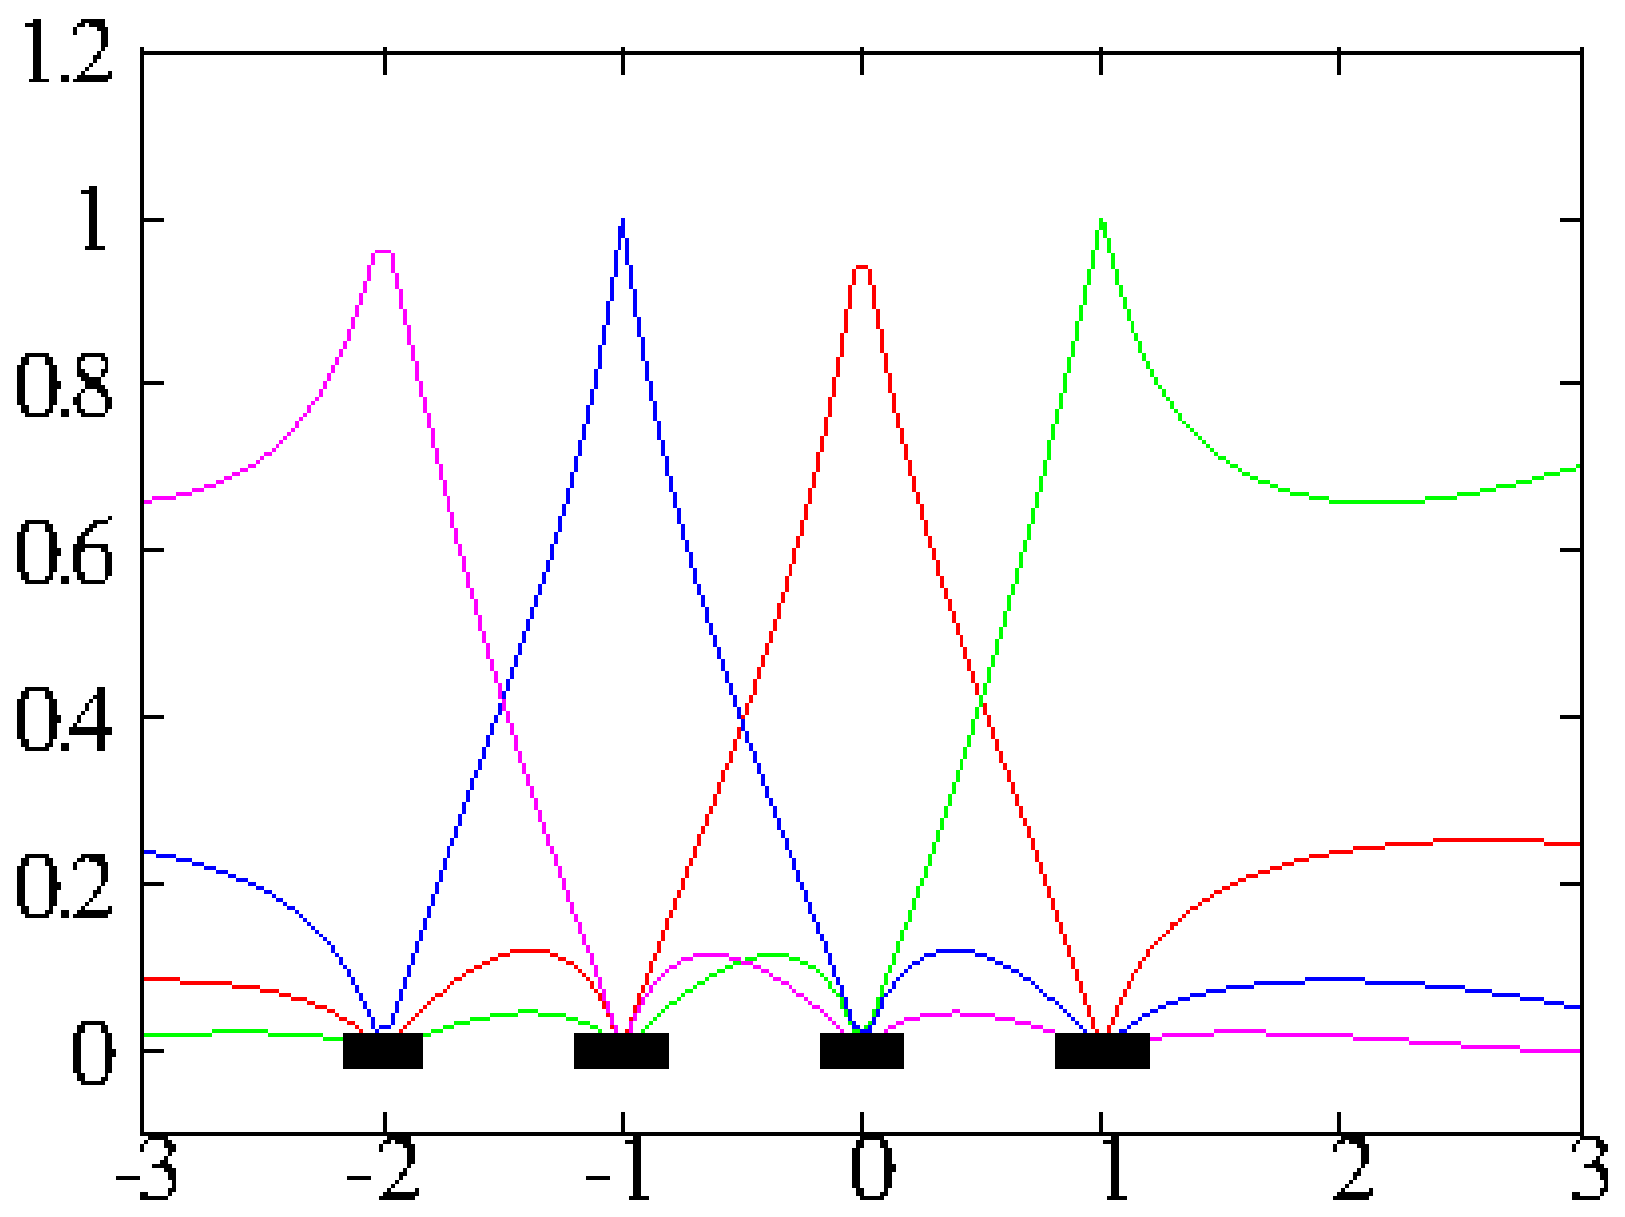
\includegraphics[scale=0.153]{./ElemShepard1.eps} &
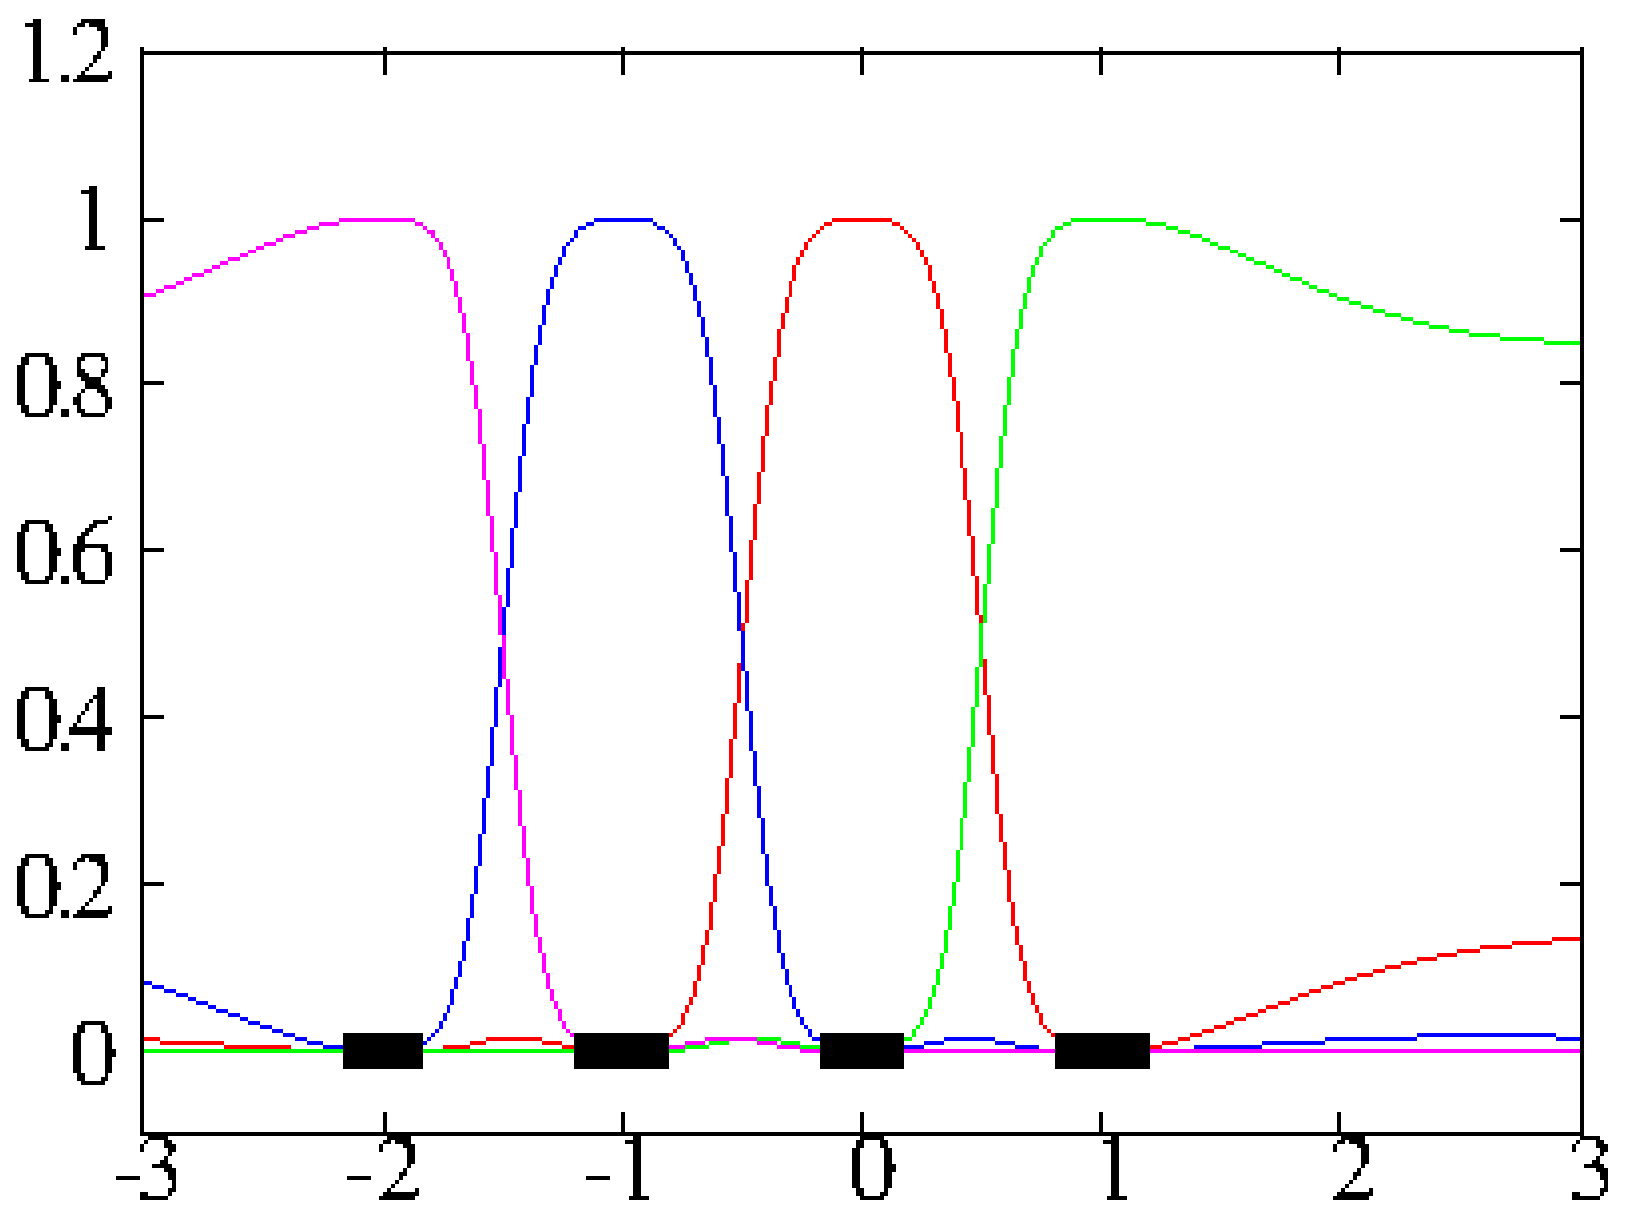
\includegraphics[scale=0.153]{./ElemShepard3.eps} \\ 
(a) & (b)\\
\end{tabular}\newline
\begin{tabular}{c}
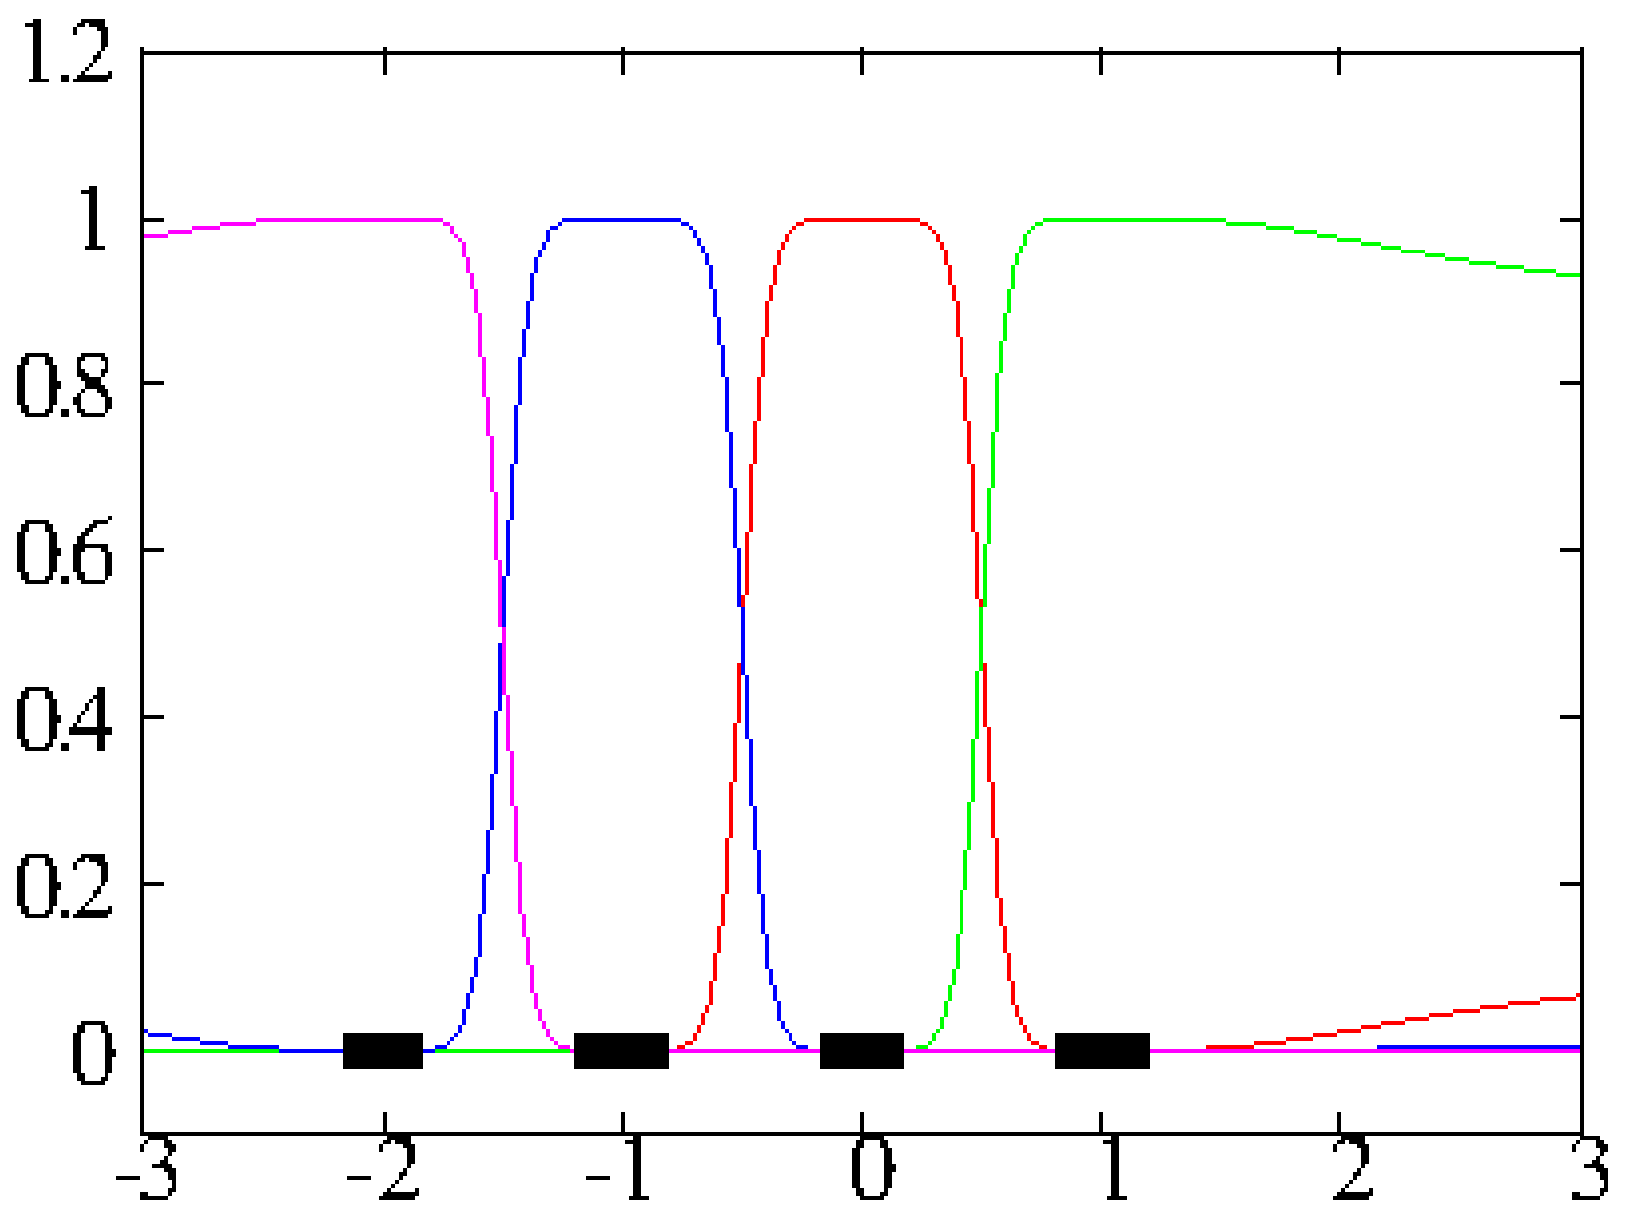
\includegraphics[scale=0.153]{./ElemShepard5.eps} \\
(c) \\
\end{tabular}
\caption{\label{fig.elemShepard}Behaviour of different Shepard bases according to three values of $k$, where the black dots stand for the center of the basis: (a) $k=1$, (b) $k=3$ and (c) $k = 5$.}
\end{figure}

Figure~\ref{fig.intShepard} depicts some interpolated functions using FEM with Shepard basis. Analogously to the behaviour of the aforementioned basis, the interpolated functions tend to become less smooth. Once more, the rectangles stand for the center of the basis.

\begin{figure}[!h]
\centering
\begin{tabular}{cc}
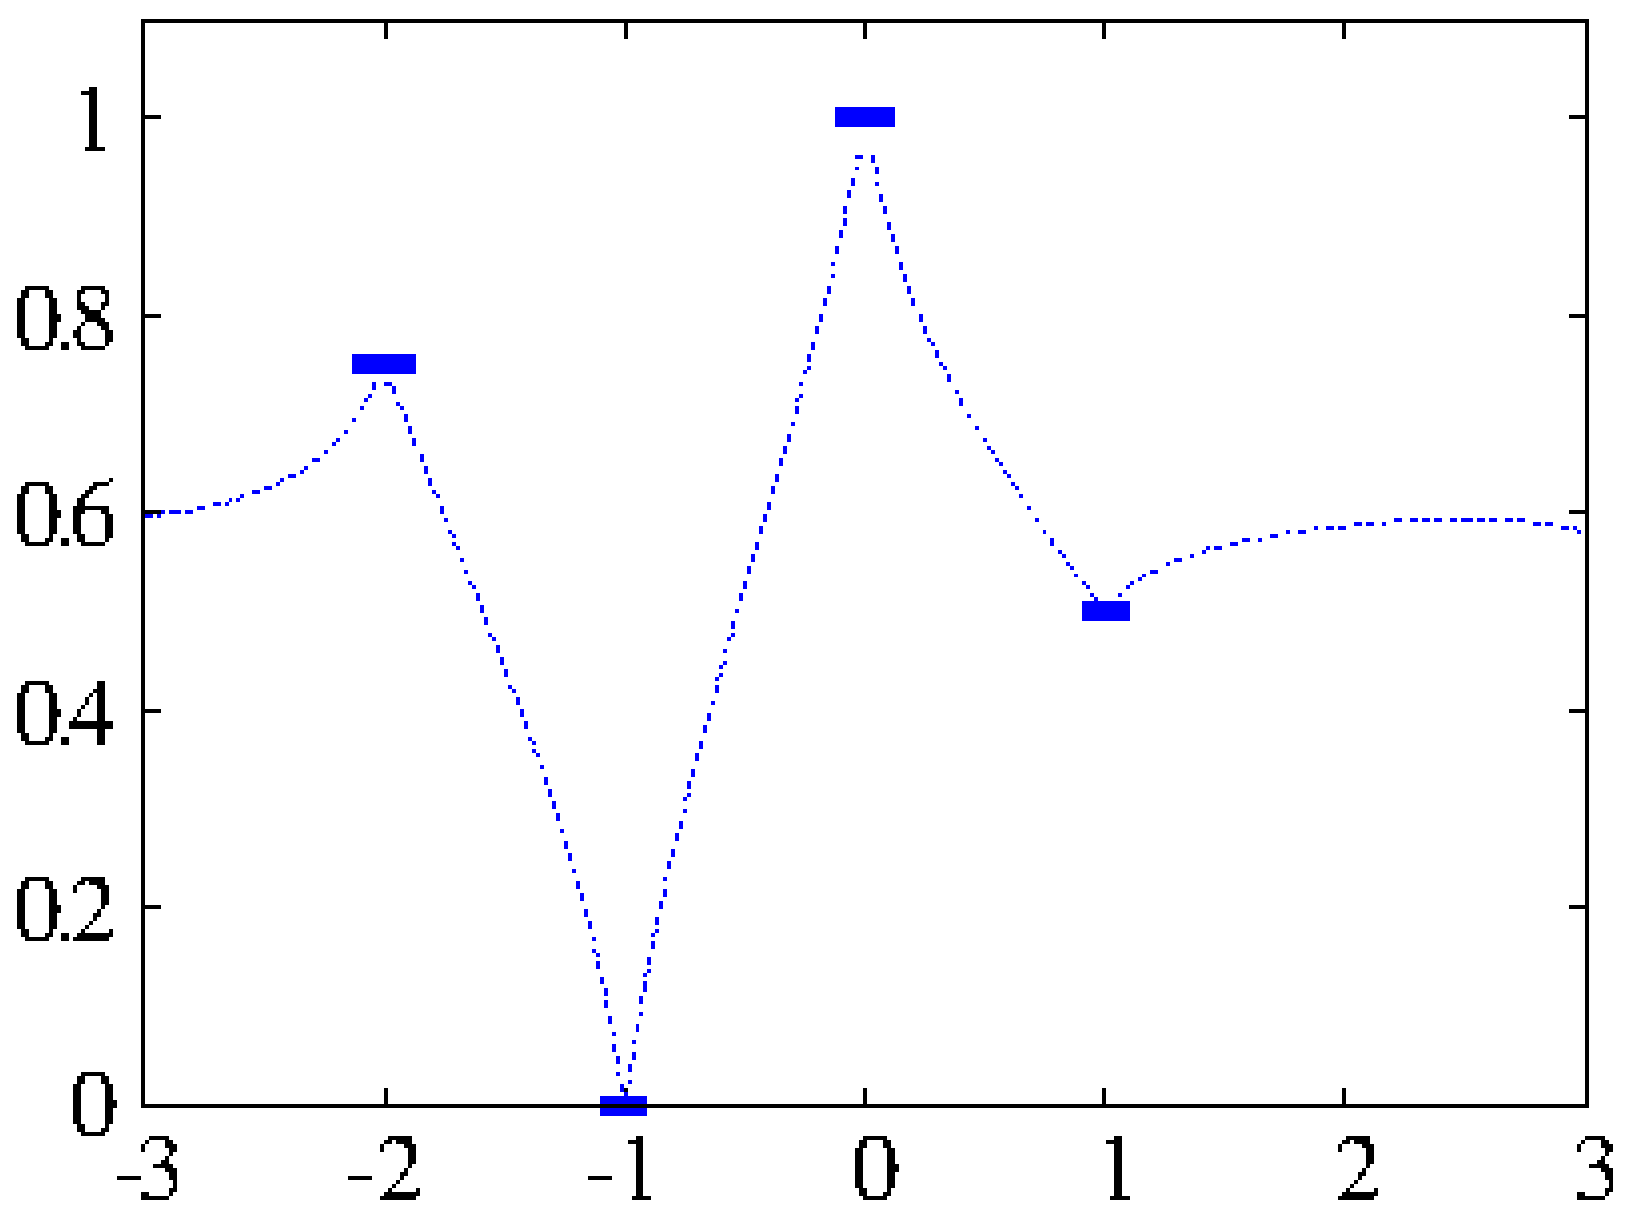
\includegraphics[scale=0.153]{./intShepard1.eps} &
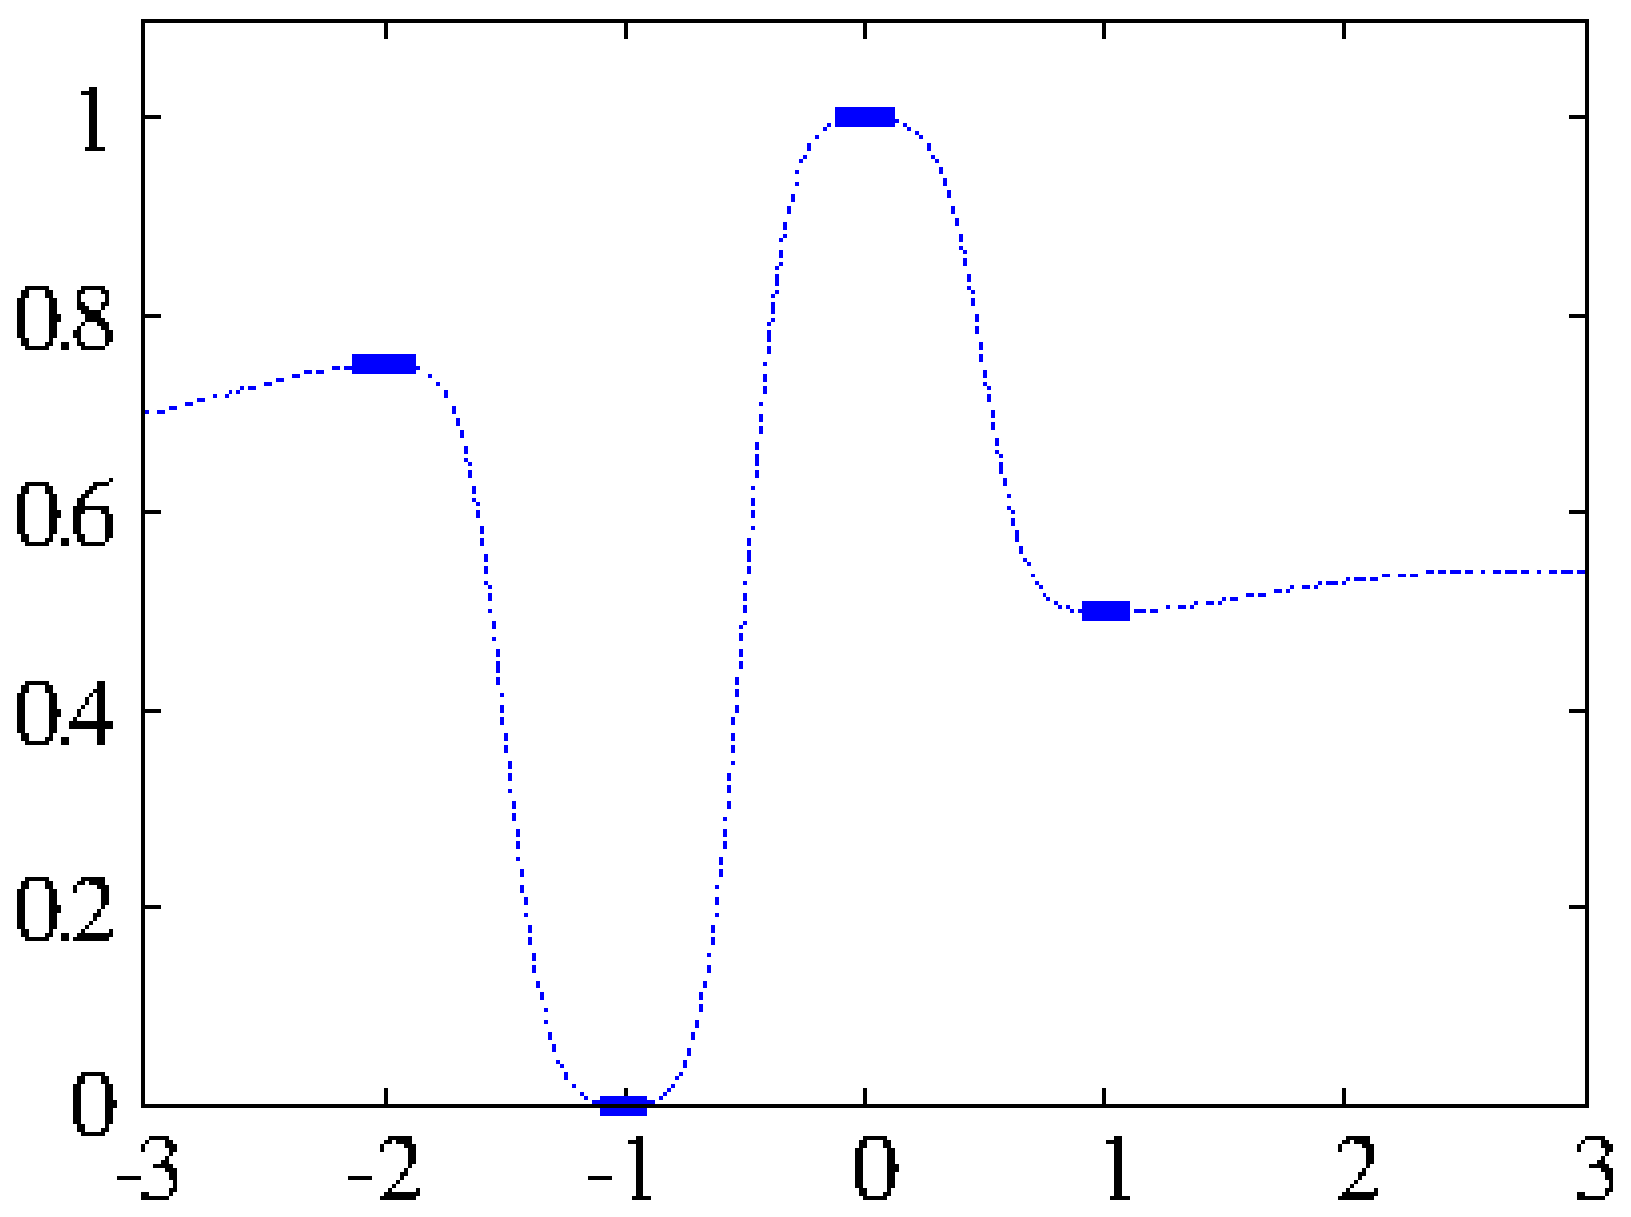
\includegraphics[scale=0.153]{./intShepard3.eps} \\ 
(a) & (b) \\
\end{tabular}
\begin{tabular}{c}
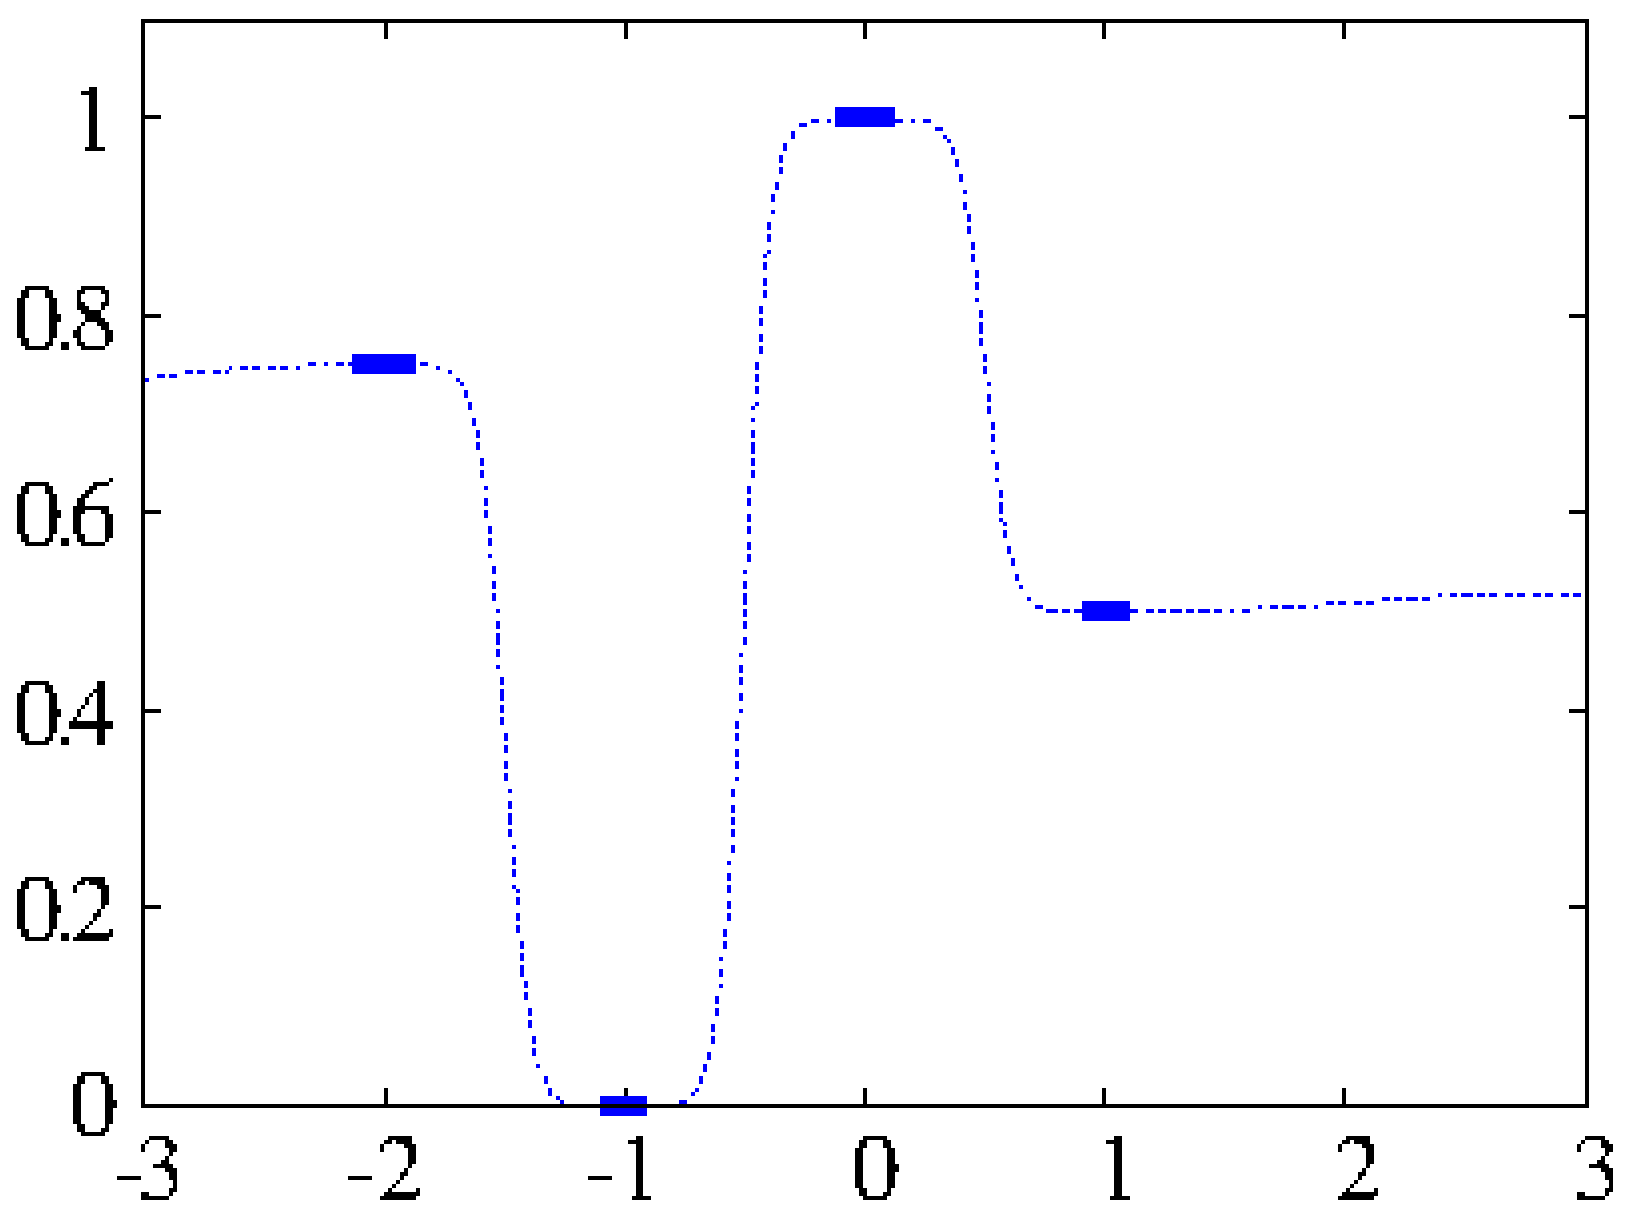
\includegraphics[scale=0.153]{./intShepard5.eps} \\
(c) \\
\end{tabular}
\caption{\label{fig.intShepard}Interpolated function using the Shepard basis for (a) $k=1$, (b) $k=3$ and (c) $k=5$. The blue rectangles represent the center of the basis and their sampled values.}
\end{figure}
\section{Finite Element Machine}
\label{s.fema}

In this section, we present the Finite Element Machine classifier, as well as how it can cope with the problem of supervised pattern classification efficiently. \textcolor{blue}{In this point is import highlight that FEMa is not a generalization of the variation o k-NN (k-Nearest Neighbour) or w-NN (Weighted Nearest Neighbour)~\cite{Samworth:12} even w-NN can being seen as an special case of the FEMa. So it is very important emphasize that FEMa has all fundamental background based on Finite Element Method . The FEMa allows work with a huge number of different basis, as: Radial Basis Function, Normalized Radial Basis Function and many others. All the background developed in this work provides a elegant solutions for basis which are neither interpolating and not partition-unit basis.  FEMa opens a wide range of new studies of finite element bases applied in machine learning.}

\subsection{Background Theory}
\label{ss.background}

Let ${\cal Z}={\cal Z}_1\cup{\cal Z}_2$ be a dataset partitioned into a training (${\cal Z}_1$) and a test (${\cal Z}_2$) set. In this case, the pair $(\textbf{x}_i,y_i)\in{\cal Z}$ denotes the feature vector $\textbf{x}_i\in\Re^m$ extracted from sample $i$, and $y_i$ stands for its label. Notice we adopted the very same formulation used in the previous section, i.e. a point in FEM formulation stands for a sample in FEMa.

Roughly speaking, FEMa learns a set of probability functions ${\cal P}(\textbf{x})=\{P_1(\textbf{x}),P_2(\textbf{x}),\ldots,P_c(\textbf{x})\}$, where $c$ stands for the number of classes, and $P_i(\textbf{x})$ represents the probability of a given sample $\textbf{x}$ to be assigned to class $i$. In other words, FEMa aims at learning a probabilistic manifold from the training set.

\subsection{Probabilistic Manifold Learning}
\label{ss.manifold}

Depending on the basis function used to interpolate points, FEMa does not require a training step, which turns out to be quite interesting when dealing with big data. Precisely, this assumption is true concerning bases that are natively interpolating, such as Shepard basis. On the other hand, with respect to non-interpolating basis, e.g. radial functions, one needs to compute $\textbf{Z}^{-1}$ in Equation~\ref{e.interpolating_basis}. Also, if the basis function does not hold the partition of unity property, one shall compute Equation~\ref{e.normalization} either. Therefore, although FEMa can be used with any basis function, we shed light over that bases holding both the interpolating and partition of unity properties are much more appealing when dealing with massive amount of data. As such, we can consider the calculation of $\textbf{Z}^{-1}$ and Equation~\ref{e.normalization} as the training steps when using non-interpolating and non-partition of units bases.

Assuming we are using an interpolating and partition of unity basis (e.g Shepard), we can move to the classification step. Given a sample $\textbf{x}\in{\cal Z}_2$, we need to compute its probability of belonging to each class $i$, $i=1,2,\ldots,c$, as follows:

\begin{equation}
	P_i(\textbf{x})=\sum_{j=1}^{\left|{\cal Z}_1\right|}\rho_i^j\phi_j(\textbf{x}),
\end{equation}
where $\rho_i^j\in[0,1]$ stands for the probability of training sample $j$ belonging to class $i$. An interesting property concerning FEMa relates to the possibility in assigning a probability to each training sample, which means we have an uncertainty associated to those samples, thus having an important role when dealing with data overfitting. This capability is extremely important in medical-driven applications, where physicians usually have different opinions with respect to the very same data (e.g. cancer detection in images).

The probability $\rho_i^j\in[0,1]$ can be computed using the following formulation:

\begin{equation}
\rho_i^j =  \left\{
			  \begin{array}{ll}
			      1 & \hbox{if $y_{j} = i$}\\
			      0 & \hbox{otherwise.}\\
			  \end{array}
		    \right.
\end{equation}
Since we have labeled datasets (i.e. we are assuming the labeling process is errorless), we can use $\rho_i^j\in\{0,1\}$. Therefore, we generate the set of probabilities ${\cal P}(\textbf{x})$ for each sample $\textbf{x}\in{\cal Z}_2$. 

In short, FEMa classifies a given sample $\textbf{x}\in{\cal Z}_2$ as belonging to the class $\hat{y}$ that satisfies the above equation:

\begin{equation}
	\hat{y} = \arg\max_{i}P_i(\textbf{x}).
\end{equation}
Also, FEMa allows us to infer the certainty $C(\textbf{x})$ as follows:

\begin{equation}
\label{eq.certainty}
	C(\textbf{x})=\frac{P_{\hat{y}}(\textbf{x})}{\sum_{j=1}^cP_j(\textbf{x})}.
\end{equation}
Therefore, FEMa can produce both hard and soft (probability) outputs without any modification. Figure~\ref{fig.ProbFunc} illustrates the process of learning the probability functions of each class in a one-dimensional and two-class problem. For the sake of explanation, the $x$-axis stands for a test set with samples within the interval $[-3,3]$, and the $y$-axis denotes their probability values with respect to the class $1$ (Figure~\ref{fig.ProbFunc}a) and class $2$ (Figure~\ref{fig.ProbFunc}b). Also, the red dots stand for the training samples, i.e. the centers of the basis functions.

Let us consider a test sample with value $-2$ in Figure~\ref{fig.ProbFunc}c. As one can observe, such sample has been used as a center for the basis function in Figure~\ref{fig.ProbFunc}a already (it is a training sample). In this case, the classification process will assign class $1$ to this sample, since $P_1(-2)\approx 1$, and $P_2(-2)\approx 0$. Now, consider a sample with value $2$ that does not belong to the training set, i.e. it is not a basis center. In this case, $P_1(2)\approx 0.15$ and $P_2(2)\approx 0.85$, which leads FEMa to assign class $2$ to that sample.

\begin{figure}[!htb]
\centering
\begin{tabular}{cc}
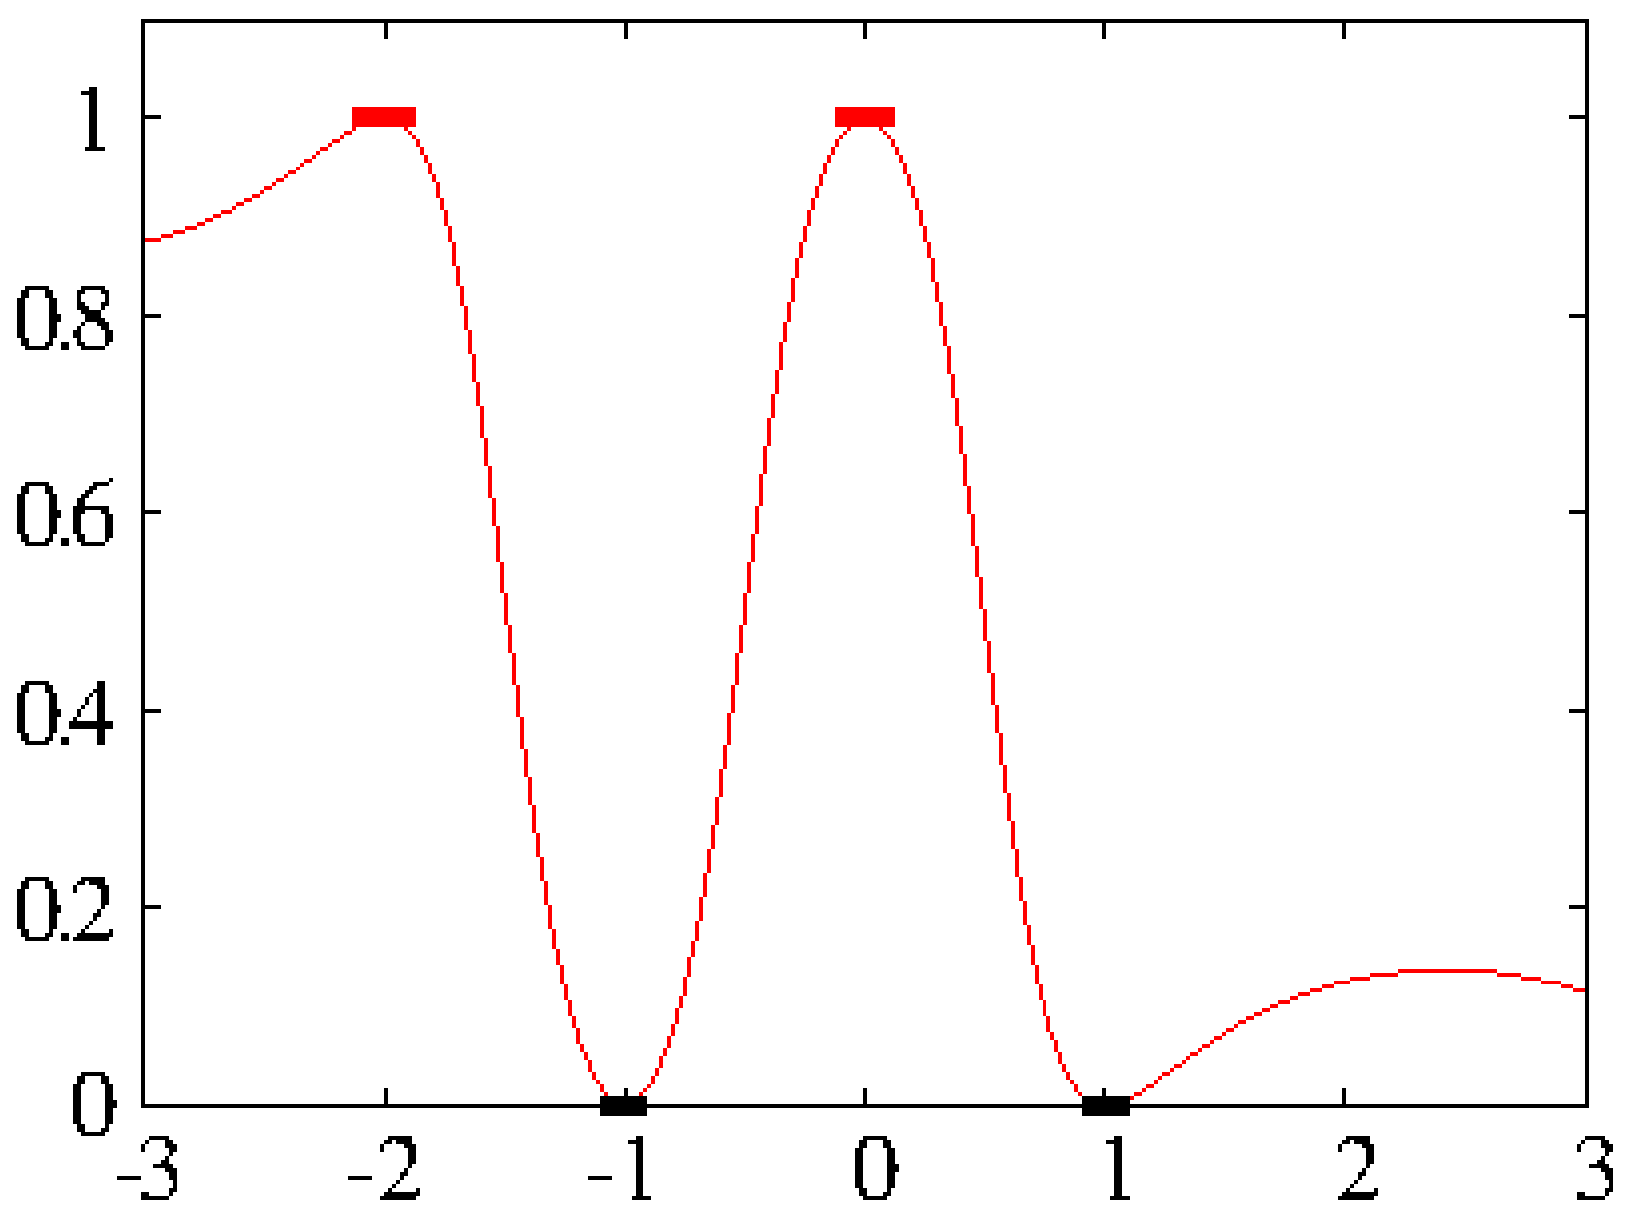
\includegraphics[scale=0.153]{./ShepardClass1.eps} &
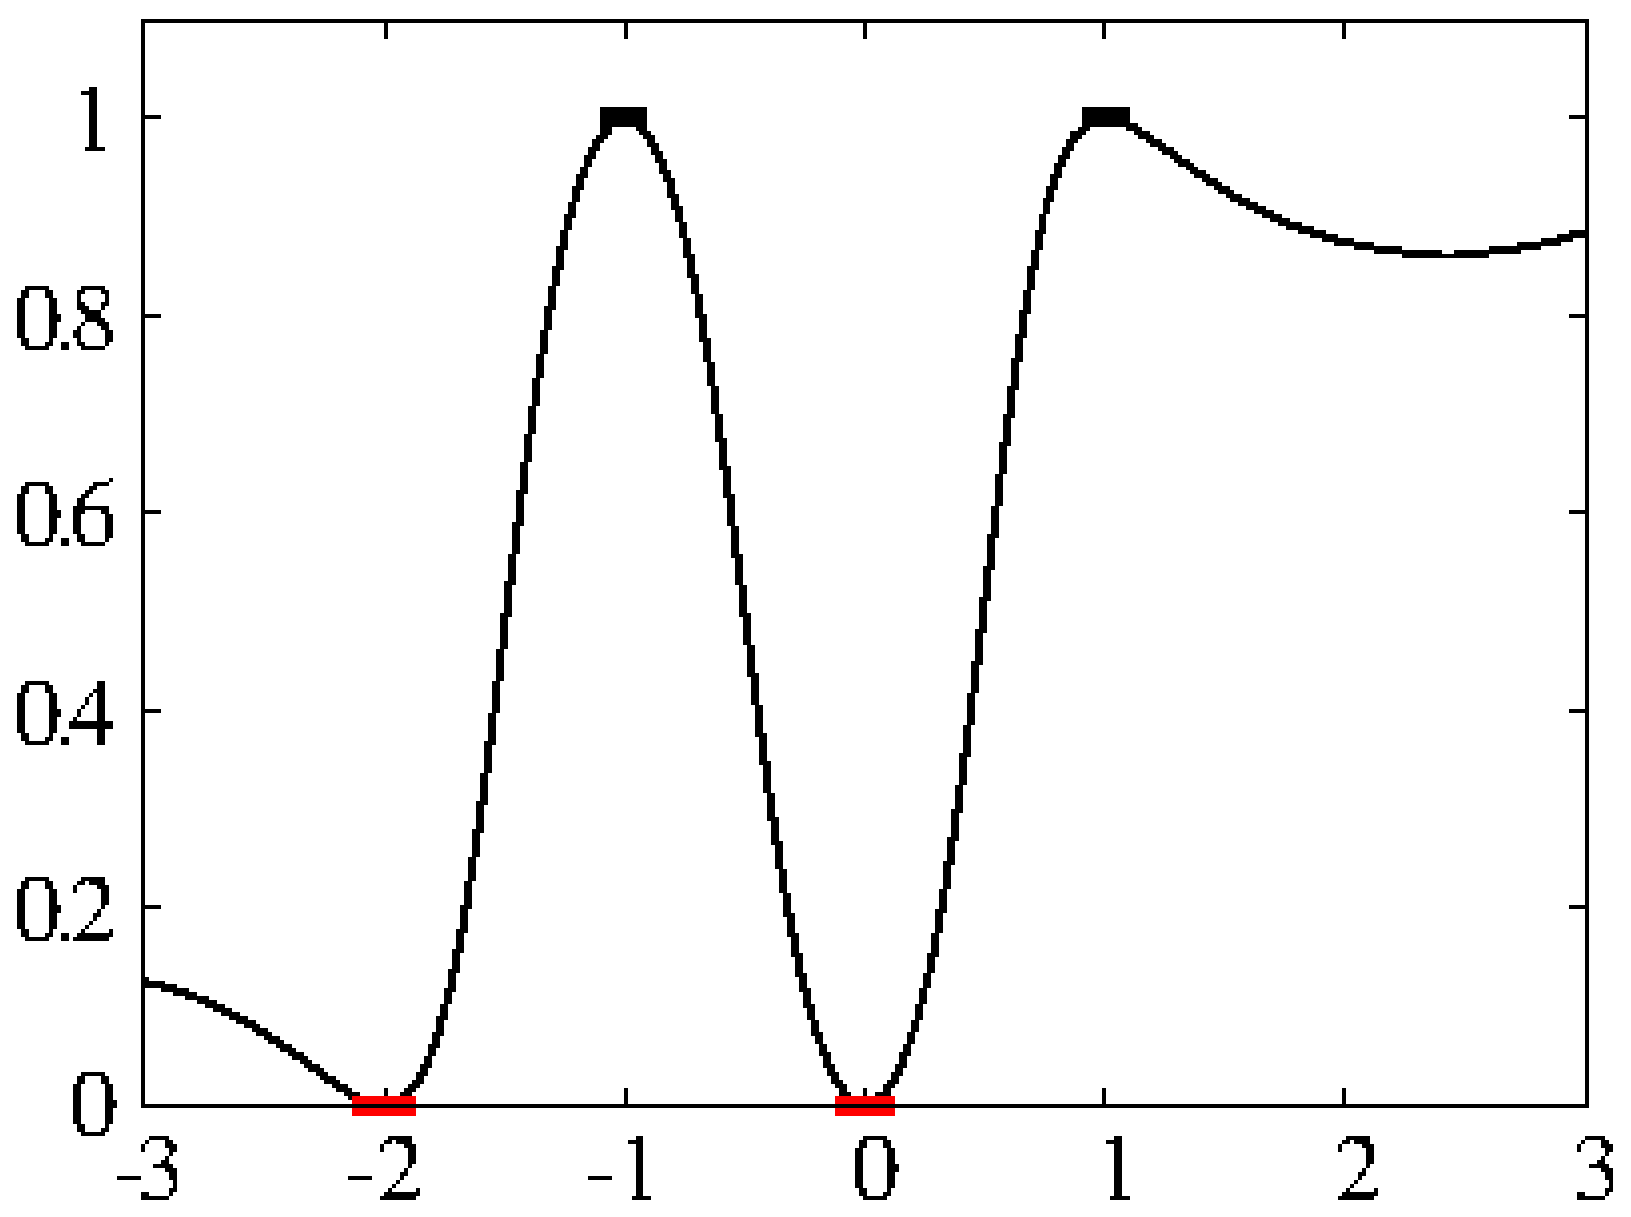
\includegraphics[scale=0.153]{./ShepardClass2.eps} \\
(a) & (b)\\
\end{tabular}
\begin{tabular}{c}
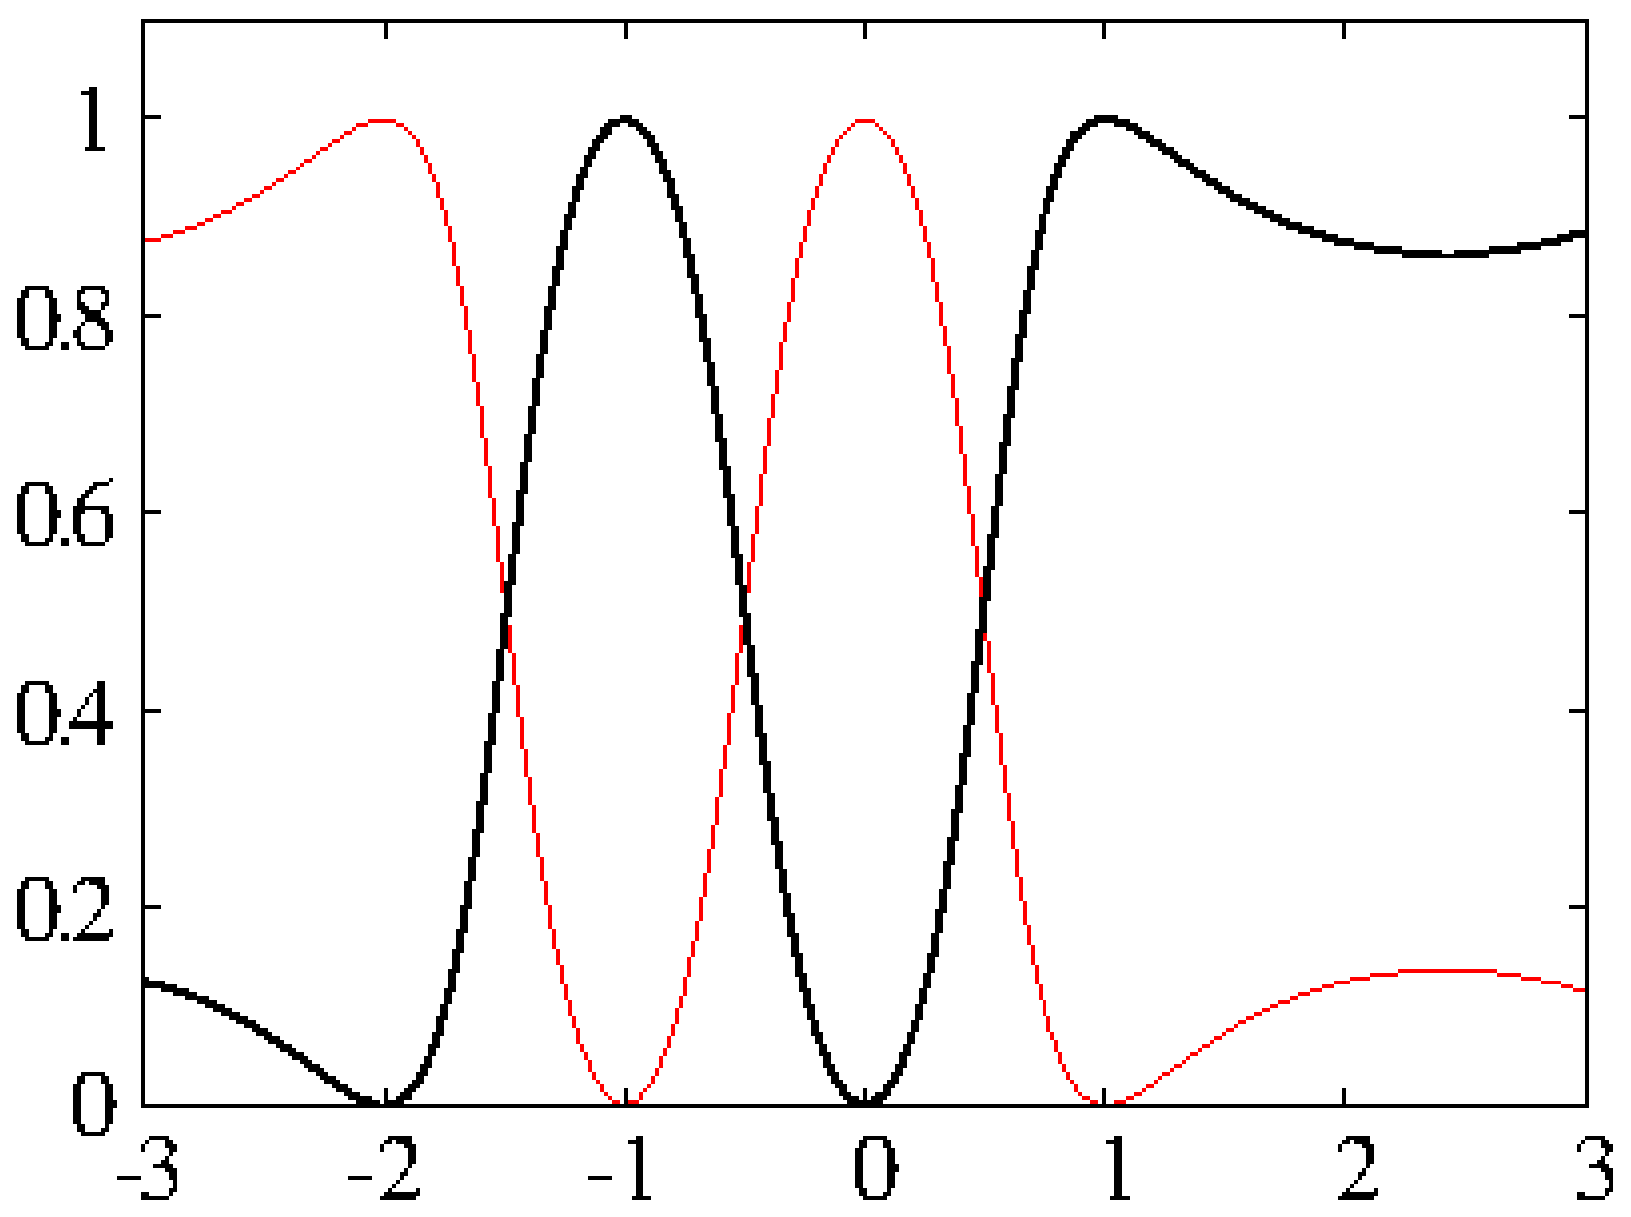
\includegraphics[scale=0.153]{./ShepardProbClass.eps} \\
(c)
\end{tabular}
\caption{The Shepard approximation of the probability function of a two-class problem using $k=3$ considering a given sample $\textbf{x}$: (a) $P_1(\textbf{x})$ and (b) $P_2(\textbf{x})$. The red dots and the red curve denote the samples and the probability function of class $1$, respectively, and the black dots and the black curve stand for the samples and the probability function of class $2$, respectively. In (c), we have the two probability functions together. Notice each real number in $[-3,3]$ (i.e. $x$-axis) is classified according to the class that has the higher probability value (i.e. $y$-axis).}
\label{fig.ProbFunc}
\end{figure}

\subsection{Toy Example}
\label{ss.toy}

In this section, we present the FEMa working mechanism on a bidimensional classification problem. Figure~\ref{2Dpoints}a shows a training set with samples distributed over three classes (red, green and blue). The task is to verify the influence region of each training sample in the image domain, i.e. to classify the remaining points (white ones) in the image frame displayed in Figure~\ref{2Dpoints}a. In this case, the feature of each sample (point) is just its $(x,y)$-position.

\begin{figure}[!htb]
\centering
\begin{tabular}{cc}
\hspace{0.31cm}\moldura{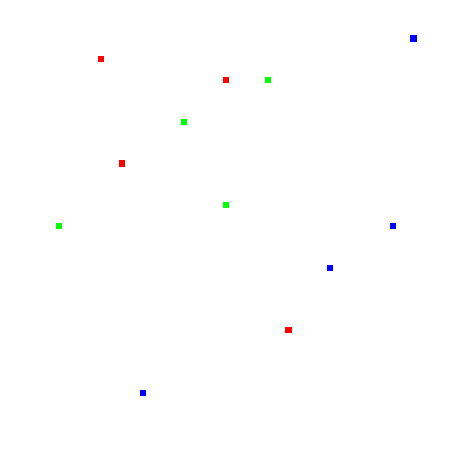
\includegraphics[width=3.39cm]{./points.eps}} &
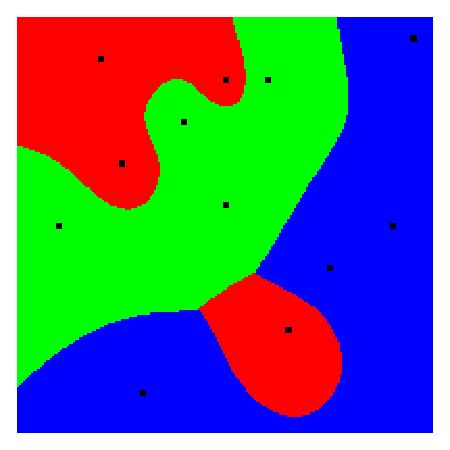
\includegraphics[width=3.39cm]{./out_p1.eps} \\
(a) & (b)\\
\end{tabular}\newline
\begin{tabular}{cc}
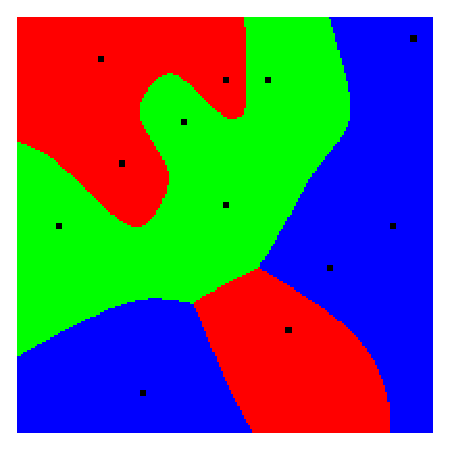
\includegraphics[width=3.39cm]{./out_p3.eps} &
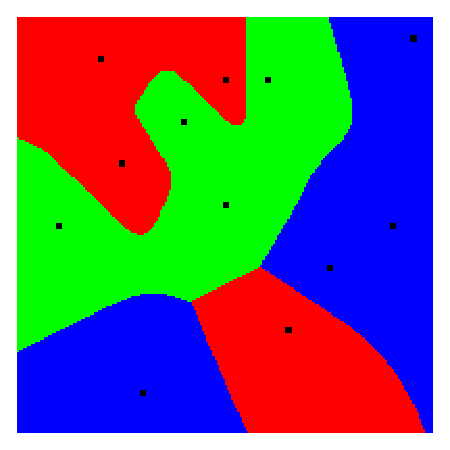
\includegraphics[width=3.39cm]{./out_p5.eps} \\
(c) & (d)\\
\end{tabular}
\caption{FEMa working mechanism: (a) training set with samples distributed in three classes, and the image classified by FEMa using (b) $k=1$, (c) $k=3$ and (d) $k=5$.}
\label{2Dpoints}
\end{figure}

Figures~\ref{2Dpoints}b,~\ref{2Dpoints}c and~\ref{2Dpoints}d depict the image frame classified by FEMa using the Shepard basis with $k=1$, $k=3$ and $k=5$, respectively. Since we are using the $(x,y)$ coordinates to describe each sample, the labeled image refers to the influence region of each training sample, which ends up generating the boundaries of each class. Notice that FEMa can obtain quite good and smooth decision boundaries for different values of $k$ (Equation~\ref{eq.w}). As matter of fact, the larger the value of $k$, the less points will influence the interpolating process of the probability function. For the sake of clarification purposes, when $k\to\infty$, FEMa tends to behave similarly to the well-known nearest neighbor classifier.

Figure~\ref{fig.2Dcertain}a displays the degree of certainty (Equation~\ref{eq.certainty}) computed by FEMa with $k=3$ for each test sample with respect to Figure~\ref{2Dpoints}a. The brighter the pixel, the greater its degree of certainty to be assigned to some class. Notice the darker pixels fall in the boundary among classes (Figure~\ref{2Dpoints}c). Figure~\ref{fig.2Dcertain}b represents each test sample by its label color weighted by its degree of certainty.

\begin{figure}[!htb]
\centering
\begin{tabular}{cc}
 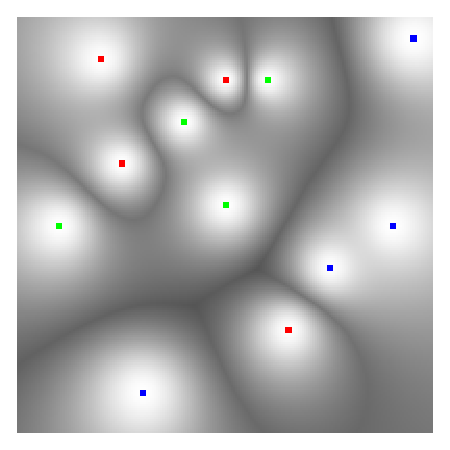
\includegraphics[scale=0.5]{./certain_p.eps} &
 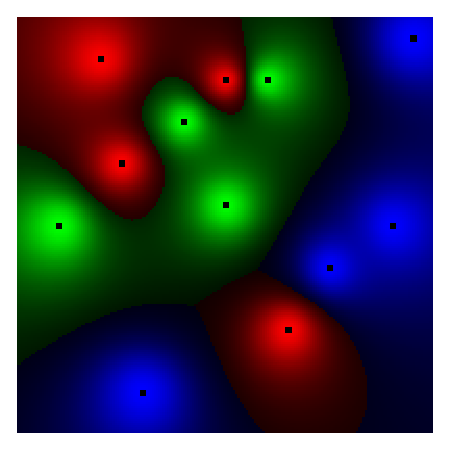
\includegraphics[scale=0.5]{./out_w_p.eps} \\
 (a) & (b)
 \end{tabular} 
 \caption{Probability map (degree of certainty) computed by FEMa in (a), and the test samples with their class label weighted by their respective degree of certainty.}
   \label{fig.2Dcertain}
\end{figure}

\subsection{Complexity Analysis}
\label{ss.complexity}

As aforementioned, depending on the basis function used to build the probabilistic manifold (i.e. interpolating and partition of unity properties), FEMa does not require an explicit training step, since we just need to place the training points, thus taking $\theta(1)$. However, if one uses a non-interpolating basis function, we need to compute the inverse matrix $\textbf{Z}^{-1}$ in Equation~\ref{e.interpolating_basis}, which requires $\theta(\left|{\cal Z}_1\right|^{2.37})$ using the Coppersmith-Winograd algorithm~\cite{Coppersmith:90}.

In regard to the classification phase, for each test sample $\textbf{x}$, we need to compute Equation~\ref{eq.shepard_basis}, which requires $\theta({\left|{\cal Z}_1\right|})$. However, the denominator of such equation considers all training samples, thus becoming a constant, and we need to compute it only once. Since the test set contains $\left|{\cal Z}_2\right|$ samples, the overall classification phase takes $\theta(\left|{\cal Z}_1\right|+\left|{\cal Z}_1\right|\left|{\cal Z}_2\right|)\in\theta(\left|{\cal Z}_1\right|.\left|{\cal Z}_2\right|)$. Therefore, by using an interpolating basis function, the whole FEMa learning and classification processes require a quadratic complexity with respect to the training/testing set size (i.e. when $\left|{\cal Z}_1\right|=\left|{\cal Z}_2\right|$).

However, when we have unbalanced datasets, samples from the majority classes will have a stronger influence when computing the probability functions. Suppose a two-class classification problem, i.e. we have samples from the positive and negative samples. Also, suppose samples from the negative class comprise only $1\%$ of the number of positive samples. When we are computing the probability function of test sample, the positive samples will play a major role during this computation process. In order to overcome this problem, we can use only the $T$ nearest training samples from each class, where $T\in O(\alpha)$ and $\alpha$ stands for the number of elements from the smallest class\footnote{In this paper, we use $T=\alpha$.}. In this case, since we need to sort the training samples according to their distances for each test sample, the classification phase now takes $\theta((\left|{\cal Z}_1\right|\log\left|{\cal Z}_1\right|).\left|{\cal Z}_2\right|)$. Notice we can make it better by using some special data structures, such as kd-trees, which require $\theta(\left|{\cal Z}_1\right|\log\left|{\cal Z}_1\right|)$ for loading the whole data only once during training. Now, with respect to the classification phase, we do not need the sorting step, since to obtain the nearest $T$ samples takes $O(T.\log\left|{\cal Z}_1\right|)$, and thus the classification phase requires $\theta((T.\log\left|{\cal Z}_1\right|).\left|{\cal Z}_2\right|)$.
\section{Experiments}
\label{s.methodology}

In this section, we present the methodology and the experiments used to asses the robustness and efficiency of FEMa against 9 other classifiers: (i) ANN trained with Backpropation, (ii) Bayes, (iii) EPNN, (iv) OPF, (v) $k$-NN ($k$-nearest neighbors), (vi) SVM with Radial Basis Function (SVM-RBF), (vii) SVM with a sigmoid function (SVM-Sigmoid), (viii) Decision Trees (DT), and (ix) Random Forest (RF). Such approaches were selected for comparison purposes since they have been commonly applied in a number of classification tasks in the literature, being some of them referred as state-of-the-art by the machine learning community.

In order to validate the experiments, we employed $23$ public benchmarking datasets\footnote{\url{http://www.csie.ntu.edu.tw/~cjlin/libsvmtools/datasets}} that have been frequently used for the evaluation of supervised classification methods. We divided the dataset into two groups: (i) small datasets and (ii) medium-to-large datasets. Tables~\ref{tab.datasets1} and~\ref{tab.datasets2} present the main characteristics of the datasets concerning the small and the medium-to-large group, respectively. The datasets were selected in order to represent distinct scenarios, which comprise datasets with different number of features, sizes and classes. 

\begin{table}[!htb]		    
\begin{center}
\caption{\label{tab.datasets1}Information about the small datasets used in the experiments.}
\small
\begin{tabular}{  l | c | c | c }
    \textbf{Dataset}   & \textbf{\# samples} & \textbf{\# features}  & \textbf{\# classes}\\ \hline \hline
    australian        &      690           &       14             &    2 \\
    boat              &      100           &       2              &    3 \\
    breast            &      683           &       10             &    2 \\      
    cone-torus       &      400           &       2              &    3 \\
    data1             &      1,423          &       2              &    2 \\
    data2             &      283           &       2              &    2 \\
    data3             &      340           &       2              &    5 \\
    data4             &      698           &       2              &    3 \\
    data5             &      1,850          &       2              &    2 \\
    diabetes          &      768           &       8              &    2 \\
    fourclass         &      862           &       2              &    2 \\
    glass             &	 214	       &       9              &    6 \\ 		        
    heart             &      270           &       13             &    2 \\   
    petals            &      100           &       2              &    4 \\  
    saturn            &      200           &       2              &    2 \\
    segment           &      2,310          &       19             &    7 \\			
    vehicle           &      846           &       18             &    4 \\ 
    wine              &      178           &       13             &    3 \\ \hline  		 
\end{tabular}		    	    
\end{center}		    
\end{table}

\begin{table}[!htb]		    
\begin{center}
\caption{\label{tab.datasets2}Information about the medium-to-large datasets used in the experiments.}
\small
\begin{tabular}{  l | c | c | c | c }
    \textbf{Dataset}   & \textbf{\# training} & \textbf{\# testing} & \textbf{\# features}  & \textbf{\# classes}\\
    & \textbf{samples} & \textbf{samples} & &\\ \hline \hline
    a1a                &  1,605                     &     30,956                & 123                & 2               \\  
    a2a                &  2,265                     &     30,296                & 123                & 2               \\
    a3a                &  3,185                     &     29,376                & 123                & 2               \\
    a4a                &  4,781                     &     27,780                & 123                & 2               \\
    a5a                &  6,414                     &     26,147                & 123                & 2               \\ \hline		        
\end{tabular}		    	    
\end{center}		    
\end{table}

Since the medium-to-large datasets are partitioned into training and testing sets already, we decided to partition the small datasets at random using $50\%$ for training purposes and the remaining $50\%$ for classification. Notice the aforementioned protocol was repeated for both normalized and non-normalized versions of the datasets under $15$ runnings for the computation of mean accuracy and computational load. The idea is to verify the behavior of FEMa under such circumstance. The normalization process is the same adopted by LibOPF~\cite{LibOPF:14}, which is used to implement the OPF classifier:

\begin{equation}
\hat{f}_i = \frac{(f_i - \tilde{f}_i)}{s_i}, 
\end{equation}
where $f_i$, $\tilde{f}_i$ and $s_i$ are, respectively, the $i$-th feature, the average of $f_i$, and the standard deviation of $f_i$ in the dataset. Also, $\hat{f}_i$ stands for the normalized version of $f_i$. In order to compare the classification methods, we computed the mean accuracy and standard deviation for each one. Further, we employed the Wilcoxon signed-rank test~\cite{Wilcoxon:45} with significance of $0.05$ to provide a more robust statistical evaluation. 

Methods that require fine-tuning parameters (i.e. SVM, $k$-NN and EPNN) are optimized differently. In regard to SVM, for Radial Basis Function and Sigmoid kernel, the searching range of parameter $C$ (optimization function) was defined within the interval $[-32, 32]$, while the searching range of parameter $\gamma$ (variance of the Gaussian kernel) was defined within the interval $[0, 32]$. For both parameters we used a step size of $2$. With respect to $k$-NN, we defined the value of $k$ as the best value of an exhaustive search in the range $[1,|{\cal{Z}}_{1}|]$ with step size of $2$ (i.e. the best value of $k$ is the one that maximizes the accuracy over the training set). For the EPNN classifier, the search space of parameter $\sigma$ (variance of the Gaussian function used in the pattern layer) was defined within $[0,1]$ with step size of $0.05$, and the search space for the radius was defined within $[l_d,m_d]$, where $l_d$ and $m_d$ denote the lowest and greatest distance among two samples. The ANN architecture employs $4$ hidden layers with $8$ neurons on each, and the number of epochs and desired error were defined as $70,000$ and $0.0001$, respectively. Concerning Random Forest we set the number of estimators to $10$, and the maximum depth to $20$. For Decision Tree we used 10-levels of depth.

\subsection{Small-sized Datasets}
\label{ss.small}

Table~\ref{tab.ACC_1} presents the mean recognition rates using $50\%$ of the datasets for training purposes with feature normalization, where the most accurate results according to the Wilcoxon statistical tool are in bold. One can observe that FEMa obtained the best results in $8$ out of $18$ datasets, being the sole best technique in two situations (i.e. ``data2'' and ``wine''). Additionally, concerning six datasets (``data1'',  ``data3'', ``data4'', ``data5'', ``fourclass'' and ``petals''), FEMa obtained recognition rates quite close to the best ones. The worst performance appears to be in the ``diabetes'' dataset, but the same has happened to all classifiers, except for ANN, which obtained the best results for this dataset so far.


%TESTING 0.5 1
\begin{sidewaystable}
% \begin{table*}[!htb]
\centering
\caption{\label{tab.ACC_1}Accuracy using 50\% of the samples for training with normalized features.}
\scriptsize
\begin{tabular}{l||l|l|l|l|l|l|l|l|l|l|}
Dataset & ANN & Bayes & OPF & EPNN & k-NN & FEMa & DT & RF &SVM-RBF & SVM-Sigmoid \\ \hline
australian& $81.37\pm2.45$& $78.93\pm1.65$& $60.27\pm4.14$& $73.14\pm1.99$& $83.86\pm2.17$& $82.16\pm1.91$& $81.40\pm2.18$& $84.53\pm1.57$& $\mathbf{85.33\pm1.09}$& $\mathbf{85.46\pm1.06}$\\ 
boat& $87.35\pm13.06$& $98.38\pm1.80$& $50.88\pm10.40$& $98.09\pm1.62$& $\mathbf{99.78\pm0.41}$& $97.79\pm1.77$& $94.56\pm3.02$& $94.41\pm3.28$& $\mathbf{99.85\pm0.44}$& $78.68\pm3.73$\\ 
breast& $\mathbf{97.18\pm1.29}$& $93.71\pm0.90$& $89.22\pm4.67$& $66.97\pm4.68$& $95.85\pm0.61$& $94.13\pm1.05$& $93.10\pm1.37$& $95.90\pm1.31$& $96.38\pm0.44$& $96.82\pm0.79$\\ 
cone& $73.07\pm2.90$& $86.97\pm1.43$& $51.53\pm10.08$& $79.71\pm1.84$& $\mathbf{88.87\pm0.49}$& $86.76\pm1.65$& $86.35\pm1.67$& $86.69\pm1.79$& $86.80\pm2.33$& $76.95\pm1.76$\\ 
data1& $95.69\pm3.29$& $\mathbf{99.49\pm0.24}$& $41.97\pm13.97$& $\mathbf{99.45\pm0.25}$& $\mathbf{99.46\pm0.24}$& $\mathbf{99.51\pm0.24}$& $99.05\pm0.40$& $98.93\pm0.47$& $\mathbf{99.49\pm0.23}$& $94.60\pm0.52$\\ 
data2& $97.85\pm0.81$& $97.98\pm0.70$& $52.43\pm4.88$& $97.63\pm0.85$& $97.91\pm0.77$& $\mathbf{98.32\pm0.16}$& $97.47\pm0.73$& $97.88\pm0.30$& $97.67\pm0.80$& $97.44\pm0.54$\\ 
data3& $95.39\pm4.29$& $98.16\pm0.85$& $51.32\pm4.14$& $98.35\pm1.33$& $\mathbf{99.23\pm0.82}$& $\mathbf{99.31\pm0.73}$& $\mathbf{99.34\pm0.71}$& $\mathbf{99.29\pm0.62}$& $\mathbf{99.27\pm0.46}$& $\mathbf{99.30\pm0.49}$\\ 
data4& $99.87\pm0.21$& $\mathbf{100.0\pm0.00}$& $70.56\pm5.75$& $\mathbf{100.0\pm0.00}$& $\mathbf{100.0\pm0.00}$& $\mathbf{100.0\pm0.00}$& $99.86\pm0.26$& $99.98\pm0.06$& $\mathbf{100.0\pm0.00}$& $\mathbf{100.0\pm0.00}$\\ 
data5& $\mathbf{100.0\pm0.00}$& $\mathbf{100.0\pm0.00}$& $48.23\pm4.34$& $99.29\pm1.52$& $\mathbf{100.0\pm0.00}$& $\mathbf{100.0\pm0.00}$& $94.29\pm2.86$& $90.24\pm4.19$& $\mathbf{100.0\pm0.00}$& $50.00\pm0.00$\\ 
diabetes& $\mathbf{72.30\pm1.25}$& $65.85\pm0.87$& $56.58\pm5.30$& $51.58\pm1.00$& $69.61\pm1.87$& $65.73\pm2.58$& $66.08\pm2.77$& $69.93\pm1.97$& $70.38\pm2.03$& $69.39\pm1.41$\\ 
fourclass& $70.92\pm1.95$& $\mathbf{99.90\pm0.21}$& $49.88\pm6.04$& $98.84\pm0.56$& $\mathbf{99.91\pm0.20}$& $\mathbf{99.91\pm0.21}$& $97.27\pm1.14$& $98.45\pm0.67$& $\mathbf{99.91\pm0.19}$& $71.05\pm2.01$\\ 
glass& $62.89\pm3.74$& $76.81\pm2.73$& $67.26\pm2.46$& $65.37\pm1.25$& $76.81\pm2.73$& $70.00\pm8.91$& $74.16\pm4.38$& $\mathbf{78.61\pm1.28}$& $76.46\pm3.30$& $73.67\pm4.28$\\ 
heart& $77.97\pm4.80$& $77.95\pm1.55$& $71.15\pm2.83$& $69.78\pm2.39$& $82.87\pm2.09$& $81.03\pm2.15$& $73.33\pm3.93$& $78.05\pm2.36$& $\mathbf{84.03\pm1.00}$& $81.75\pm2.73$\\ 
petals& $98.72\pm1.52$& $99.36\pm0.64$& $51.41\pm4.60$& $99.23\pm0.85$& $99.36\pm0.64$& $\mathbf{99.76\pm0.48}$& $96.67\pm1.64$& $96.54\pm1.82$& $99.49\pm0.63$& $\mathbf{99.74\pm0.51}$\\ 
saturn& $63.40\pm13.02$& $89.00\pm3.61$& $58.30\pm8.27$& $\mathbf{90.12\pm1.06}$& $89.00\pm3.61$& $88.70\pm4.05$& $86.30\pm2.83$& $85.90\pm2.84$& $88.60\pm2.20$& $49.20\pm4.92$\\ 
segment& $66.55\pm3.74$& $97.07\pm0.18$& $89.03\pm0.67$& $96.92\pm0.22$& $97.07\pm0.18$& $96.96\pm0.16$& $96.78\pm0.47$& $\mathbf{98.20\pm0.24}$& $97.64\pm0.31$& $96.93\pm0.27$\\ 
vehicle& $67.33\pm4.14$& $79.46\pm1.13$& $65.52\pm1.53$& $78.91\pm0.84$& $79.82\pm1.06$& $80.03\pm0.92$& $79.28\pm1.60$& $82.42\pm0.84$& $\mathbf{88.27\pm0.74}$& $86.12\pm1.34$\\ 
wine& $95.53\pm2.43$& $96.01\pm0.96$& $71.46\pm2.58$& $93.97\pm2.91$& $96.46\pm1.28$& $\mathbf{98.49\pm0.62}$& $94.43\pm2.51$& $97.52\pm0.89$& $98.16\pm1.05$& $97.11\pm1.60$\\ 
\end{tabular}
% \end{table*}
\end{sidewaystable}


Table~\ref{tab.ACC_0} presents the mean recognition rates with non-normalized features. Once again, FEMa obtained the best results in $11$ out $18$ datasets, being the sole best technique in one situation (i.e. ``wine''). Additionally, concerning ten datasets (``boat'', ``cone'', ``data1'', ``data2'',  ``data3'', ``data4'', ``data5'', ``fourclass'', ``petals'' and ``segment''), FEMa obtained recognition rates quite close to the best ones.

%TESTING 0.5 1
\begin{sidewaystable}
% \begin{table*}[!htb]
\centering
\caption{\label{tab.ACC_0}Accuracy using 50\% of the samples for training with non-normalized features.}
\scriptsize
\begin{tabular}{l||l|l|l|l|l|l|l|l|l|l|}
Dataset & ANN & Bayes & OPF & EPNN & k-NN & FEMa & DT & RF &SVM-RBF & SVM-Sigmoid \\ \hline
australian& $77.48\pm6.85$& $79.41\pm1.51$& $50.38\pm5.14$& $76.49\pm1.98$& $\mathbf{86.17\pm1.21}$& $81.86\pm1.02$& $82.42\pm1.33$& $83.49\pm1.92$& $\mathbf{86.51\pm1.29}$& $\mathbf{86.90\pm1.59}$\\ 
boat& $93.38\pm4.84$& $97.65\pm1.76$& $49.26\pm6.75$& $98.53\pm1.32$& $97.65\pm1.76$& $\mathbf{99.59\pm0.71}$& $96.03\pm3.16$& $95.88\pm1.84$& $\mathbf{99.71\pm0.88}$& $76.03\pm2.94$\\ 
breast& $50.04\pm0.13$& $55.19\pm2.19$& $95.83\pm0.35$& $52.68\pm0.48$& $53.80\pm2.33$& $75.32\pm2.20$& $93.54\pm1.67$& $\mathbf{96.13\pm1.14}$& $50.93\pm0.68$& $50.00\pm0.00$\\ 
cone& $77.05\pm14.59$& $\mathbf{87.78\pm1.99}$& $85.21\pm1.50$& $84.12\pm2.60$& $\mathbf{88.24\pm1.60}$& $\mathbf{87.95\pm1.76}$& $85.24\pm1.63$& $\mathbf{87.83\pm2.03}$& $\mathbf{87.98\pm3.17}$& $75.94\pm1.17$\\ 
data1& $99.16\pm0.46$& $99.40\pm0.13$& $99.22\pm0.24$& $99.32\pm0.33$& $\mathbf{99.56\pm0.20}$& $\mathbf{99.67\pm0.21}$& $99.03\pm0.40$& $\mathbf{98.68\pm0.52}$& $99.39\pm0.29$& $94.16\pm0.57$\\ 
data2& $88.33\pm19.20$& $\mathbf{98.57\pm0.54}$& $97.33\pm1.44$& $\mathbf{98.50\pm0.58}$& $\mathbf{98.63\pm0.69}$& $\mathbf{98.61\pm0.74}$& $\mathbf{98.51\pm0.82}$& $97.62\pm1.17$& $\mathbf{98.56\pm0.80}$& $85.38\pm2.46$\\ 
data3& $63.43\pm6.99$& $\mathbf{99.68\pm0.49}$& $\mathbf{99.72\pm0.70}$& $91.58\pm1.36$& $\mathbf{99.75\pm0.27}$& $\mathbf{99.78\pm0.49}$& $99.46\pm0.54$& $98.76\pm0.80$& $\mathbf{99.65\pm0.44}$& $98.05\pm1.35$\\ 
data4& $81.70\pm18.21$& $\mathbf{100.0\pm0.00}$& $\mathbf{100.0\pm0.00}$& $99.96\pm0.08$& $\mathbf{100.0\pm0.00}$& $\mathbf{100.0\pm0.00}$& $99.91\pm0.26$& $\mathbf{100.0\pm0.00}$& $99.97\pm0.09$& $50.00\pm0.00$\\ 
data5& $64.99\pm22.90$& $\mathbf{100.0\pm0.00}$& $\mathbf{100.0\pm0.00}$& $74.40\pm0.60$& $\mathbf{100.0\pm0.00}$& $\mathbf{100.0\pm0.00}$& $96.90\pm3.38$& $89.52\pm5.85$& $99.76\pm0.71$& $50.00\pm0.00$\\ 
diabetes& $59.55\pm8.05$& $67.82\pm1.52$& $59.67\pm5.90$& $51.64\pm0.34$& $69.29\pm1.85$& $66.53\pm1.22$& $67.53\pm1.49$& $\mathbf{71.64\pm1.32}$& $\mathbf{71.62\pm1.22}$& $\mathbf{71.72\pm1.59}$\\ 
fourclass& $75.28\pm11.81$& $\mathbf{99.88\pm0.30}$& $46.72\pm6.91$& $98.93\pm0.87$& $99.60\pm0.30$& $\mathbf{99.92\pm0.13}$& $97.52\pm0.63$& $98.78\pm0.71$& $\mathbf{99.95\pm0.12}$& $71.29\pm1.77$\\ 
glass& $62.32\pm6.37$& $76.87\pm4.58$& $48.57\pm2.39$& $65.32\pm2.10$& $76.87\pm4.58$& $61.38\pm6.14$& $75.66\pm3.39$& $76.35\pm2.39$& $\mathbf{78.46\pm2.27}$& $72.18\pm4.28$\\ 
heart& $78.72\pm3.57$& $76.25\pm4.11$& $58.53\pm7.41$& $73.12\pm2.61$& $82.92\pm2.57$& $81.73\pm2.69$& $75.32\pm2.17$& $78.87\pm2.11$& $\mathbf{83.37\pm1.46}$& $\mathbf{83.28\pm1.85}$\\ 
petals& $98.85\pm1.46$& $\mathbf{99.62\pm0.59}$& $52.18\pm4.59$& $\mathbf{99.56\pm0.86}$& $\mathbf{99.62\pm0.59}$& $\mathbf{99.62\pm0.59}$& $96.67\pm2.24$& $96.79\pm1.31$& $99.23\pm0.85$& $99.23\pm0.85$\\ 
saturn& $59.90\pm10.59$& $89.30\pm3.38$& $51.80\pm7.37$& $89.00\pm3.49$& $89.30\pm3.38$& $88.80\pm2.82$& $85.40\pm4.32$& $87.10\pm4.23$& $\mathbf{91.60\pm1.56}$& $48.20\pm4.98$\\ 
segment& $66.18\pm7.31$& $97.41\pm0.30$& $66.88\pm1.07$& $97.38\pm0.31$& $97.41\pm0.30$& $\mathbf{98.01\pm0.38}$& $96.80\pm0.52$& $\mathbf{97.92\pm0.29}$& $97.40\pm0.43$& $96.83\pm0.47$\\ 
vehicle& $69.13\pm6.83$& $78.21\pm0.90$& $54.66\pm2.82$& $79.21\pm1.10$& $78.25\pm0.62$& $79.79\pm1.33$& $78.85\pm0.96$& $82.42\pm0.95$& $\mathbf{88.11\pm0.98}$& $85.78\pm1.27$\\ 
wine& $95.67\pm1.77$& $96.83\pm1.22$& $46.45\pm4.03$& $94.30\pm2.50$& $97.39\pm1.17$& $\mathbf{98.79\pm0.72}$& $92.21\pm3.47$& $97.49\pm1.43$& $98.00\pm1.17$& $98.10\pm1.38$
\end{tabular}
% \end{table*}
\end{sidewaystable}


%TESTING 0.5 1
\begin{sidewaystable}
% \begin{table*}[!htb]
\centering
\caption{\label{tab.TIME_0_TR}Mean training time using 50\% of the samples for training without normalized features.}
\scriptsize
\begin{tabular}{l||l|l|l|l|l|l|l|l|l|}
Dataset & ANN & Bayes & OPF & EPNN & k-NN & DT & RF &SVM-RBF & SVM-Sigmoid \\ \hline
australian& $70.8734\pm20.8491$& $0.0032\pm0.0032$& $0.0052\pm0.0016$& $31.1273\pm31.8675$& $0.2606\pm0.2192$& $0.0211\pm0.0198$& $0.1263\pm0.0957$& $18.7846\pm2.8732$& $19.1068\pm10.0762$\\ 
boat& $0.7629\pm2.0788$& $0.0000\pm0.0000$& $0.0001\pm0.0000$& $0.2113\pm0.2139$& $0.0002\pm0.0000$& $0.0034\pm0.0032$& $0.0824\pm0.0822$& $0.7586\pm0.0552$& $0.8130\pm0.0676$\\ 
breast& $63.2710\pm4.4166$& $0.0018\pm0.0027$& $0.0058\pm0.0011$& $105.6959\pm107.6519$& $0.1763\pm0.1795$& $0.0155\pm0.0118$& $0.1068\pm0.1037$& $11.7905\pm1.1035$& $4.7998\pm0.6750$\\ 
cone& $34.9401\pm1.0360$& $0.0002\pm0.0000$& $0.0012\pm0.0012$& $3.8731\pm3.9213$& $0.0115\pm0.0005$& $0.0048\pm0.0056$& $0.0642\pm0.0465$& $5.3449\pm0.6784$& $2.9298\pm0.8012$\\ 
data1& $120.9207\pm9.2261$& $0.0038\pm0.0016$& $0.0124\pm0.0050$& $41.4977\pm41.6274$& $2.3441\pm0.6390$& $0.0150\pm0.0160$& $0.1152\pm0.1065$& $26.9878\pm3.0218$& $18.9863\pm1.5381$\\ 
data2& $25.0916\pm1.1162$& $0.0002\pm0.0000$& $0.0009\pm0.0002$& $1.4743\pm1.4822$& $0.0089\pm0.0023$& $0.0045\pm0.0042$& $0.1056\pm0.0872$& $1.9385\pm0.2096$& $1.4296\pm0.1284$\\ 
data3& $39.2747\pm0.6773$& $0.0003\pm0.0000$& $0.0011\pm0.0002$& $2.3249\pm2.3279$& $0.0120\pm0.0004$& $0.0065\pm0.0060$& $0.1056\pm0.0707$& $3.8453\pm0.2585$& $2.3549\pm0.0870$\\ 
data4& $34.6149\pm33.7621$& $0.0012\pm0.0003$& $0.0047\pm0.0009$& $10.8775\pm10.8804$& $0.1934\pm0.0352$& $0.0111\pm0.0095$& $0.1132\pm0.1007$& $9.4711\pm0.4358$& $6.7878\pm0.3496$\\ 
data5& $127.9521\pm58.2196$& $0.0025\pm0.0001$& $0.0330\pm0.0073$& $73.1067\pm73.1002$& $7.1692\pm0.2125$& $0.0171\pm0.0141$& $0.1343\pm0.1211$& $34.9273\pm0.4245$& $3.5497\pm0.1981$\\ 
diabetes& $76.9009\pm7.7117$& $0.0029\pm0.0031$& $0.0064\pm0.0021$& $16.2853\pm16.4400$& $0.3225\pm0.1056$& $0.0350\pm0.0273$& $0.1456\pm0.1265$& $48.5885\pm4.3913$& $11.9431\pm1.3355$\\ 
fourclass& $53.0143\pm24.6785$& $0.0012\pm0.0004$& $0.0043\pm0.0010$& $19.0229\pm19.0328$& $0.3755\pm0.0873$& $0.0162\pm0.0126$& $0.0838\pm0.0765$& $16.8570\pm1.5027$& $10.1930\pm0.5919$\\ 
glass& $27.7234\pm0.8222$& $0.0002\pm0.0000$& $0.0005\pm0.0001$& $1.7531\pm1.7704$& $0.0028\pm0.0001$& $0.0125\pm0.0105$& $0.1138\pm0.0803$& $2.9637\pm0.2638$& $2.3756\pm0.2353$\\ 
heart& $8.6923\pm12.6581$& $0.0003\pm0.0001$& $0.0017\pm0.0002$& $2.9456\pm3.1076$& $0.0088\pm0.0014$& $0.0160\pm0.0126$& $0.1202\pm0.0739$& $3.2283\pm0.3567$& $2.9895\pm0.2867$\\ 
petals& $0.4466\pm1.2274$& $0.0000\pm0.0000$& $0.0001\pm0.0000$& $0.2820\pm0.2894$& $0.0002\pm0.0000$& $0.0031\pm0.0008$& $0.0841\pm0.0187$& $0.7951\pm0.0597$& $0.7669\pm0.0847$\\ 
saturn& $15.6057\pm0.6604$& $0.0001\pm0.0000$& $0.0003\pm0.0000$& $1.1707\pm1.1713$& $0.0021\pm0.0003$& $0.0136\pm0.0045$& $0.0723\pm0.0120$& $3.4344\pm0.4841$& $1.4702\pm0.2089$\\ 
segment& $358.3062\pm4.4535$& $0.0420\pm0.0037$& $0.1336\pm0.0242$& $68.2178\pm14.1303$& $17.9593\pm0.4701$& $0.1989\pm0.1844$& $0.2493\pm0.0545$& $133.1311\pm6.5640$& $141.9412\pm3.2699$\\ 
vehicle& $112.9792\pm2.3228$& $0.0061\pm0.0020$& $0.0137\pm0.0017$& $39.8968\pm40.7552$& $0.4687\pm0.0431$& $0.0650\pm0.0638$& $0.1489\pm0.0447$& $35.5804\pm1.9432$& $27.1175\pm1.1371$\\ 
wine& $0.0590\pm0.0196$& $0.0002\pm0.0000$& $0.0007\pm0.0001$& $0.5427\pm0.5471$& $0.0021\pm0.0003$& $0.0094\pm0.0075$& $0.0865\pm0.0169$& $1.4247\pm0.1644$& $1.1740\pm0.0403$
\end{tabular}
% \end{table*}
\end{sidewaystable}

%TESTING 0.5 1
\begin{sidewaystable}
% \begin{table*}[!htb]
\centering
\caption{\label{tab.TIME_1_TR}Mean training time using 50\% of the samples for training with normalized features.}
\scriptsize
\begin{tabular}{l||l|l|l|l|l|l|l|l|l|}
Dataset & ANN & Bayes & OPF & EPNN & k-NN & DT & RF &SVM-RBF & SVM-Sigmoid \\ \hline
australian& $68.8698\pm12.2983$& $0.0024\pm0.0007$& $0.0166\pm0.0019$& $29.1966\pm29.6731$& $0.2221\pm0.0503$& $0.0317\pm0.0277$& $0.1039\pm0.0219$& $20.1067\pm2.3381$& $15.6099\pm5.2604$\\ 
boat& $2.7584\pm4.0748$& $0.0000\pm0.0000$& $0.0001\pm0.0000$& $0.2566\pm0.2574$& $0.0002\pm0.0000$& $0.0040\pm0.0034$& $0.0735\pm0.0225$& $1.0913\pm0.0940$& $1.1831\pm0.1008$\\ 
breast& $58.6247\pm19.4740$& $0.0015\pm0.0004$& $0.0116\pm0.0032$& $50.9665\pm51.2110$& $0.1931\pm0.0326$& $0.0183\pm0.0189$& $0.0920\pm0.0195$& $7.3862\pm0.6035$& $3.8115\pm0.3425$\\ 
cone& $33.7404\pm0.4724$& $0.0003\pm0.0002$& $0.0010\pm0.0002$& $4.6924\pm4.7137$& $0.0199\pm0.0035$& $0.0085\pm0.0068$& $0.0704\pm0.0187$& $8.8075\pm1.1684$& $3.2669\pm0.3826$\\ 
data1& $67.1394\pm50.5443$& $0.0044\pm0.0012$& $0.0115\pm0.0029$& $46.6753\pm46.6847$& $2.6932\pm0.2489$& $0.0143\pm0.0109$& $0.0947\pm0.0244$& $13.6852\pm0.8035$& $13.7717\pm0.5369$\\ 
data2& $0.0401\pm0.0232$& $0.0001\pm0.0000$& $0.0005\pm0.0001$& $1.9648\pm1.9724$& $0.0078\pm0.0016$& $0.0044\pm0.0043$& $0.0734\pm0.0212$& $1.2987\pm0.1115$& $1.1489\pm0.0411$\\ 
data3& $18.0523\pm16.1725$& $0.0003\pm0.0001$& $0.0007\pm0.0001$& $2.8901\pm2.8898$& $0.0143\pm0.0038$& $0.0072\pm0.0064$& $0.0874\pm0.0150$& $2.1101\pm0.2198$& $2.0138\pm0.1550$\\ 
data4& $0.2133\pm0.0936$& $0.0012\pm0.0006$& $0.0029\pm0.0005$& $13.0600\pm13.0740$& $0.1655\pm0.0287$& $0.0069\pm0.0044$& $0.0842\pm0.0218$& $3.6659\pm0.3026$& $3.5820\pm0.3848$\\ 
data5& $0.5607\pm0.0957$& $0.0030\pm0.0008$& $0.0304\pm0.0081$& $83.5806\pm83.7034$& $6.3606\pm0.3573$& $0.0222\pm0.0186$& $0.0879\pm0.0292$& $10.2319\pm0.6333$& $32.0421\pm3.8786$\\ 
diabetes& $72.7618\pm3.8639$& $0.0022\pm0.0008$& $0.0145\pm0.0032$& $17.4858\pm17.4979$& $0.3058\pm0.0506$& $0.0302\pm0.0257$& $0.0917\pm0.0195$& $45.3156\pm5.5513$& $13.3924\pm0.8592$\\ 
fourclass& $66.2280\pm1.4766$& $0.0010\pm0.0000$& $0.0044\pm0.0008$& $19.7155\pm19.7218$& $0.3365\pm0.0269$& $0.0109\pm0.0087$& $0.0634\pm0.0089$& $17.4455\pm1.0236$& $10.3772\pm0.3794$\\ 
glass& $27.9809\pm0.4939$& $0.0002\pm0.0001$& $0.0010\pm0.0001$& $4.2144\pm4.3995$& $0.0033\pm0.0009$& $0.0129\pm0.0106$& $0.1548\pm0.1136$& $3.2737\pm0.2572$& $2.6343\pm0.2296$\\ 
heart& $8.7291\pm12.5433$& $0.0003\pm0.0001$& $0.0029\pm0.0003$& $1.6564\pm1.6640$& $0.0089\pm0.0017$& $0.0125\pm0.0028$& $0.1173\pm0.0992$& $3.3764\pm0.3799$& $3.1131\pm0.3787$\\ 
petals& $0.0468\pm0.0524$& $0.0000\pm0.0000$& $0.0001\pm0.0000$& $0.2966\pm0.2968$& $0.0002\pm0.0000$& $0.0053\pm0.0041$& $0.0759\pm0.0429$& $0.7997\pm0.0367$& $0.7535\pm0.0182$\\ 
saturn& $15.5077\pm0.4991$& $0.0001\pm0.0000$& $0.0003\pm0.0000$& $1.1673\pm1.1720$& $0.0022\pm0.0005$& $0.0046\pm0.0040$& $0.0966\pm0.1029$& $3.2531\pm0.2667$& $1.4456\pm0.0612$\\ 
segment& $366.1648\pm14.7373$& $0.0455\pm0.0126$& $0.2715\pm0.1775$& $1053.2818\pm1053.2457$& $18.7171\pm1.3856$& $0.1683\pm0.1575$& $0.2411\pm0.2027$& $146.4743\pm4.8722$& $101.6875\pm2.4436$\\ 
vehicle& $113.2932\pm7.6061$& $0.0055\pm0.0010$& $0.0250\pm0.0087$& $38.3586\pm38.5061$& $0.3919\pm0.0488$& $0.0654\pm0.0610$& $0.1815\pm0.1309$& $35.9961\pm3.1782$& $26.0429\pm2.5516$\\ 
wine& $0.0625\pm0.0186$& $0.0002\pm0.0000$& $0.0012\pm0.0003$& $0.5882\pm0.5948$& $0.0022\pm0.0003$& $0.0105\pm0.0019$& $0.0942\pm0.0841$& $1.4507\pm0.2065$& $1.0942\pm0.0733$
\end{tabular}
% \end{table*}
\end{sidewaystable}



Tables~\ref{tab.TIME_0_TR} and~\ref{tab.TIME_1_TR} present the mean computational load for training purposes considering normalized and non-normalized features. Notice we did not show the results concerning FEMa, since it does not have training step. The most expensive techniques are the ones that require parameter fine-tuning (i.e. $k$-NN, SVM and EPNN), since we considered the time spent on this step to the final training procedure computational load. Our implementation of the Bayesian classifier is considerably fast for training, since it basically consists into finding the maximum arc-weight among training samples to be used as a normalization factor in the exponential function (probability estimates).

%TESTING 0.5 1
\begin{sidewaystable}
% \begin{table*}[!htb]
\centering
\caption{\label{tab.TIME_0_TEST}Mean testing time using 50\% of the samples for training without normalized features.}
\scriptsize
\begin{tabular}{l||l|l|l|l|l|l|l|l|l|l|}
Dataset & ANN & Bayes & OPF & EPNN & k-NN & FEMa & DT & RF &SVM-RBF & SVM-Sigmoid \\ \hline
australian& $0.0004\pm0.0004$& $0.0121\pm0.0118$& $0.0002\pm0.0001$& $0.0501\pm0.0104$& $0.0127\pm0.0137$& $0.1377\pm0.0657$& $0.0175\pm0.0028$& $0.0197\pm0.0150$& $0.0223\pm0.0077$& $0.0300\pm0.0138$\\ 
boat& $0.0001\pm0.0000$& $0.0001\pm0.0000$& $0.0001\pm0.0000$& $0.0003\pm0.0000$& $0.0001\pm0.0000$& $0.0017\pm0.0001$& $0.0020\pm0.0003$& $0.0134\pm0.0125$& $0.0028\pm0.0001$& $0.0028\pm0.0002$\\ 
breast& $0.0003\pm0.0003$& $0.0061\pm0.0065$& $0.0026\pm0.0007$& $0.0230\pm0.0033$& $0.0031\pm0.0036$& $0.0912\pm0.0733$& $0.0121\pm0.0113$& $0.0192\pm0.0184$& $0.0258\pm0.0245$& $0.0098\pm0.0024$\\ 
cone& $0.0001\pm0.0000$& $0.0008\pm0.0000$& $0.0006\pm0.0008$& $0.0035\pm0.0001$& $0.0006\pm0.0001$& $0.0139\pm0.0011$& $0.0049\pm0.0048$& $0.0128\pm0.0089$& $0.0089\pm0.0084$& $0.0072\pm0.0076$\\ 
data1& $0.0005\pm0.0001$& $0.0231\pm0.0061$& $0.0046\pm0.0024$& $0.0516\pm0.0160$& $0.0105\pm0.0075$& $0.3210\pm0.1193$& $0.0073\pm0.0027$& $0.0228\pm0.0220$& $0.0245\pm0.0073$& $0.0393\pm0.0365$\\ 
data2& $0.0001\pm0.0000$& $0.0009\pm0.0001$& $0.0003\pm0.0001$& $0.0024\pm0.0003$& $0.0006\pm0.0004$& $0.0122\pm0.0008$& $0.0032\pm0.0005$& $0.0235\pm0.0207$& $0.0047\pm0.0007$& $0.0061\pm0.0006$\\ 
data3& $0.0002\pm0.0000$& $0.0020\pm0.0002$& $0.0004\pm0.0001$& $0.0035\pm0.0003$& $0.0008\pm0.0002$& $0.0168\pm0.0005$& $0.0034\pm0.0001$& $0.0207\pm0.0126$& $0.0054\pm0.0010$& $0.0058\pm0.0006$\\ 
data4& $0.0003\pm0.0000$& $0.0082\pm0.0019$& $0.0015\pm0.0003$& $0.0144\pm0.0013$& $0.0017\pm0.0005$& $0.0831\pm0.0097$& $0.0052\pm0.0007$& $0.0211\pm0.0173$& $0.0107\pm0.0017$& $0.0129\pm0.0049$\\ 
data5& $0.0007\pm0.0001$& $0.0417\pm0.0044$& $0.0124\pm0.0036$& $0.1134\pm0.0073$& $0.0094\pm0.0001$& $0.1638\pm0.0041$& $0.0100\pm0.0006$& $0.0272\pm0.0246$& $0.0327\pm0.0051$& $0.0068\pm0.0010$\\ 
diabetes& $0.0003\pm0.0000$& $0.0145\pm0.0169$& $0.0026\pm0.0010$& $0.0385\pm0.0077$& $0.0111\pm0.0157$& $0.1424\pm0.1282$& $0.0140\pm0.0032$& $0.0233\pm0.0206$& $0.0237\pm0.0048$& $0.0201\pm0.0049$\\ 
fourclass& $0.0003\pm0.0000$& $0.0060\pm0.0009$& $0.0005\pm0.0001$& $0.0262\pm0.0023$& $0.0027\pm0.0009$& $0.0899\pm0.0088$& $0.0057\pm0.0007$& $0.0164\pm0.0134$& $0.0057\pm0.0014$& $0.0168\pm0.0034$\\ 
glass& $0.0001\pm0.0000$& $0.0018\pm0.0005$& $0.0003\pm0.0001$& $0.0033\pm0.0002$& $0.0003\pm0.0000$& $0.0009\pm0.0002$& $0.0065\pm0.0015$& $0.0188\pm0.0145$& $0.0067\pm0.0027$& $0.0057\pm0.0009$\\ 
heart& $0.0002\pm0.0000$& $0.0013\pm0.0004$& $0.0009\pm0.0001$& $0.0072\pm0.0004$& $0.0012\pm0.0004$& $0.0198\pm0.0027$& $0.0081\pm0.0016$& $0.0215\pm0.0136$& $0.0068\pm0.0013$& $0.0056\pm0.0010$\\ 
petals& $0.0001\pm0.0000$& $0.0002\pm0.0000$& $0.0001\pm0.0000$& $0.0003\pm0.0000$& $0.0001\pm0.0000$& $0.0025\pm0.0004$& $0.0024\pm0.0004$& $0.0174\pm0.0042$& $0.0035\pm0.0008$& $0.0031\pm0.0005$\\ 
saturn& $0.0001\pm0.0000$& $0.0003\pm0.0000$& $0.0001\pm0.0000$& $0.0013\pm0.0002$& $0.0001\pm0.0000$& $0.0064\pm0.0008$& $0.0028\pm0.0005$& $0.0150\pm0.0035$& $0.0034\pm0.0005$& $0.0041\pm0.0006$\\ 
segment& $0.0015\pm0.0001$& $0.4226\pm0.0940$& $0.0662\pm0.0137$& $0.7448\pm0.0296$& $0.0452\pm0.0019$& $4.1816\pm0.1311$& $0.0930\pm0.0195$& $0.0232\pm0.0042$& $0.1265\pm0.0243$& $0.1094\pm0.0123$\\ 
vehicle& $0.0005\pm0.0000$& $0.0331\pm0.0108$& $0.0069\pm0.0012$& $0.0933\pm0.0063$& $0.0072\pm0.0014$& $0.3260\pm0.0457$& $0.0313\pm0.0011$& $0.0194\pm0.0055$& $0.0365\pm0.0045$& $0.0345\pm0.0055$\\ 
wine& $0.0001\pm0.0000$& $0.0008\pm0.0002$& $0.0005\pm0.0001$& $0.0030\pm0.0001$& $0.0004\pm0.0001$& $0.0082\pm0.0003$& $0.0053\pm0.0002$& $0.0171\pm0.0024$& $0.0051\pm0.0007$& $0.0044\pm0.0005$
\end{tabular}
% \end{table*}
\end{sidewaystable}

%TESTING 0.5 1
\begin{sidewaystable}
% \begin{table*}[!htb]
\centering
\caption{\label{tab.TIME_1_TEST}Mean testing time using 50\% of the samples for training with normalized features.}
\scriptsize
\begin{tabular}{l||l|l|l|l|l|l|l|l|l|l|}
Dataset & ANN & Bayes & OPF & EPNN & k-NN & FEMa & DT & RF &SVM-RBF & SVM-Sigmoid \\ \hline
australian& $0.0003\pm0.0000$& $0.0102\pm0.0038$& $0.0089\pm0.0012$& $0.0500\pm0.0018$& $0.0083\pm0.0029$& $0.1297\pm0.0142$& $0.0202\pm0.0030$& $0.0164\pm0.0038$& $0.0268\pm0.0067$& $0.0252\pm0.0051$\\ 
boat& $0.0001\pm0.0000$& $0.0001\pm0.0000$& $0.0001\pm0.0000$& $0.0004\pm0.0000$& $0.0001\pm0.0000$& $0.0020\pm0.0002$& $0.0028\pm0.0007$& $0.0162\pm0.0042$& $0.0035\pm0.0006$& $0.0034\pm0.0006$\\ 
breast& $0.0003\pm0.0000$& $0.0092\pm0.0016$& $0.0033\pm0.0009$& $0.0374\pm0.0015$& $0.0041\pm0.0010$& $0.0895\pm0.0103$& $0.0139\pm0.0029$& $0.0158\pm0.0032$& $0.0101\pm0.0027$& $0.0086\pm0.0027$\\ 
cone& $0.0001\pm0.0000$& $0.0014\pm0.0003$& $0.0001\pm0.0000$& $0.0054\pm0.0007$& $0.0008\pm0.0003$& $0.0230\pm0.0024$& $0.0039\pm0.0005$& $0.0143\pm0.0035$& $0.0050\pm0.0009$& $0.0060\pm0.0008$\\ 
data1& $0.0005\pm0.0001$& $0.0288\pm0.0061$& $0.0010\pm0.0003$& $0.0676\pm0.0089$& $0.0215\pm0.0091$& $0.3171\pm0.0327$& $0.0082\pm0.0016$& $0.0178\pm0.0046$& $0.0103\pm0.0048$& $0.0160\pm0.0058$\\ 
data2& $0.0001\pm0.0000$& $0.0008\pm0.0001$& $0.0001\pm0.0000$& $0.0029\pm0.0002$& $0.0005\pm0.0001$& $0.0125\pm0.0005$& $0.0031\pm0.0005$& $0.0144\pm0.0049$& $0.0038\pm0.0015$& $0.0047\pm0.0013$\\ 
data3& $0.0001\pm0.0000$& $0.0025\pm0.0008$& $0.0001\pm0.0000$& $0.0049\pm0.0010$& $0.0006\pm0.0004$& $0.0169\pm0.0021$& $0.0040\pm0.0010$& $0.0182\pm0.0023$& $0.0055\pm0.0011$& $0.0056\pm0.0015$\\ 
data4& $0.0003\pm0.0000$& $0.0101\pm0.0051$& $0.0006\pm0.0001$& $0.0186\pm0.0012$& $0.0015\pm0.0004$& $0.0749\pm0.0093$& $0.0051\pm0.0008$& $0.0158\pm0.0039$& $0.0177\pm0.0056$& $0.0191\pm0.0023$\\ 
data5& $0.0007\pm0.0001$& $0.0404\pm0.0043$& $0.0049\pm0.0020$& $0.1365\pm0.0090$& $0.0096\pm0.0021$& $0.1596\pm0.0159$& $0.0102\pm0.0020$& $0.0164\pm0.0057$& $0.0087\pm0.0026$& $0.0154\pm0.0104$\\ 
diabetes& $0.0003\pm0.0000$& $0.0086\pm0.0020$& $0.0075\pm0.0018$& $0.0446\pm0.0030$& $0.0053\pm0.0014$& $0.1049\pm0.0116$& $0.0167\pm0.0037$& $0.0149\pm0.0026$& $0.0254\pm0.0097$& $0.0244\pm0.0046$\\ 
fourclass& $0.0003\pm0.0000$& $0.0062\pm0.0005$& $0.0005\pm0.0001$& $0.0281\pm0.0021$& $0.0020\pm0.0003$& $0.0882\pm0.0016$& $0.0055\pm0.0002$& $0.0130\pm0.0018$& $0.0064\pm0.0020$& $0.0211\pm0.0037$\\ 
glass& $0.0001\pm0.0000$& $0.0020\pm0.0005$& $0.0007\pm0.0001$& $0.0036\pm0.0003$& $0.0003\pm0.0001$& $0.0010\pm0.0002$& $0.0060\pm0.0011$& $0.0297\pm0.0207$& $0.0066\pm0.0009$& $0.0067\pm0.0013$\\ 
heart& $0.0002\pm0.0000$& $0.0011\pm0.0002$& $0.0016\pm0.0001$& $0.0076\pm0.0004$& $0.0014\pm0.0005$& $0.0195\pm0.0013$& $0.0080\pm0.0007$& $0.0212\pm0.0189$& $0.0081\pm0.0012$& $0.0070\pm0.0007$\\ 
petals& $0.0001\pm0.0000$& $0.0002\pm0.0000$& $0.0001\pm0.0000$& $0.0004\pm0.0000$& $0.0001\pm0.0000$& $0.0024\pm0.0001$& $0.0023\pm0.0002$& $0.0131\pm0.0090$& $0.0033\pm0.0007$& $0.0032\pm0.0004$\\ 
saturn& $0.0001\pm0.0000$& $0.0003\pm0.0001$& $0.0001\pm0.0000$& $0.0012\pm0.0002$& $0.0001\pm0.0000$& $0.0063\pm0.0007$& $0.0027\pm0.0003$& $0.0199\pm0.0194$& $0.0031\pm0.0004$& $0.0042\pm0.0007$\\ 
segment& $0.0015\pm0.0001$& $0.3977\pm0.1212$& $0.1458\pm0.1086$& $0.7108\pm0.1007$& $0.0507\pm0.0103$& $4.3874\pm0.6432$& $0.0810\pm0.0100$& $0.0259\pm0.0214$& $0.1470\pm0.0166$& $0.1112\pm0.0173$\\ 
vehicle& $0.0004\pm0.0001$& $0.0282\pm0.0044$& $0.0214\pm0.0050$& $0.0818\pm0.0119$& $0.0060\pm0.0010$& $0.5470\pm0.4026$& $0.0280\pm0.0038$& $0.0225\pm0.0158$& $0.0369\pm0.0083$& $0.0336\pm0.0084$\\ 
wine& $0.0001\pm0.0000$& $0.0010\pm0.0002$& $0.0007\pm0.0002$& $0.0030\pm0.0003$& $0.0004\pm0.0001$& $0.0089\pm0.0012$& $0.0053\pm0.0007$& $0.0178\pm0.0164$& $0.0053\pm0.0019$& $0.0053\pm0.0021$
\end{tabular}
% \end{table*}
\end{sidewaystable}



Tables~\ref{tab.TIME_0_TEST} and~\ref{tab.TIME_1_TEST} present the mean computational load concerning the classification time over the small-sized datasets considering normalized and non-normalized features. Clearly, one can observe all techniques are considerably fast, since the datasets do not comprise so many samples. In this experiment, FEMa appears to be the slowest one, but if one considers the whole procedure (i.e. training+classification), FEMa is one of the fastest approaches, being also pretty much very accurate in a large number of situations.


\subsection{Medium-to-large-sized Datasets}
\label{ss.medium_to_large}

Table~\ref{tab.L_ACC} presents the recognition rates of the medium-to-large datasets used in this work with normalized features, where the best results according to Wilcoxon signed-rank test are in bold. In this case, SVM-RBF obtained the best results for all datasets, followed by $k$-NN and FEMa. Since the medium-sized datasets have a considerable number of samples for training purposes, SVM-RBF can benefit from that, since the samples will be mapped to a higher dimensional space for learning the maximum-marge hyperplane. However, its training step is too costly, as showed in Table~\ref{tab.L_TR_TIME}. Except for Bayes, OPF, DT, and RF, all other classifiers required a considerable computational load for training, which is prohibitive in real-time learning systems, where the training set behavior changes over time. In this situation, FEMa seems to be most suitable approach, since it does not require the training step under the interpolating and partition-of-unit assumptions.

\begin{table*}[!htb]
\begin{center}
\scriptsize
\caption{Recognition rates concerning the medium-to-large datasets.}
\label{tab.L_ACC}
\begin{tabular}{l|lllllllllllll}
Dataset & ANN     & Bayes   & EPNN    & FEMa    & $k$-NN  & OPF     &      DT  &      RF    &    SVM-RBF   & SVM-Sigmoid  \\ \hline \hline
a1a     & $81.43$ & $79.32$ & $76.10$ & $81.83$ & $82.58$ & $71.27$ & $72.22$  & $72.18$    & $\mathbf{84.05}$ &  $75.52$\\
a2a     & $81.84$ & $79.05$ & $76.15$ & $81.69$ & $82.44$ & $71.72$ & $69.51$  & $71.34$    & $\mathbf{84.06}$ &  $76.68$\\
a3a     & $79.46$ & $79.23$ & $76.08$ & $81.74$ & $82.71$ & $72.53$ & $71.31$  & $72.38$    & $\mathbf{84.45}$ &  $75.87$\\
a4a     & $81.50$ & $79.58$ & $79.73$ & $81.94$ & $83.02$ & $73.77$ & $72.43$  & $72.46$    &$\mathbf{84.56}$ &  $75.18$\\
a5a     & $82.05$ & $79.61$ & $79.56$ & $81.99$ & $83.06$ & $73.43$ & $72.57$  & $73.32$    &$\mathbf{84.49}$ &  $75.72$\\ \hline
\end{tabular}
\end{center}
\end{table*}




%training
\begin{table*}[!htb]
\begin{center}
\caption{\label{tab.L_TR_TIME}Training time concerning the medium-to-large datasets.}
\scriptsize
\begin{tabular}{l||llllllllll}
Dataset & ANN     & Bayes  & OPF   & EPNN        & $k$-NN       &      DT  &  RF    & SVM-RBF & SVM-Sigmoid  \\ \hline \hline
a1a& $ 477.41$&   $ 0.44$& $ 1.60$ & $ 7,439.90$ & $ 387.06$    & $5.47$   & $5.82$ & $ 1,130.59$ & $587.96$ \\ 
a2a& $ 706.92$&   $ 0.97$& $ 2.72$ & $ 17,758.61$& $ 813.43$    & $3.42$   & $5.56$ & $ 2,292.08$ & $1207.18$\\ 
a3a& $ 964.27$&   $ 1.38$& $ 5.76$ & $ 11,336.21$& $ 2,592.87$  & $5.26$   & $6.04$ & $ 4,557.10$ & $2603.14$\\ 
a4a& $ 1,449.42$& $ 3.75$& $ 12.68$& $ 45,847.83$& $ 10,470.55$ & $5.99$   & $6.60$ & $ 10,870.21$& $5466.43$\\ 
a5a& $ 1,926.00$& $ 6.71$& $ 24.36$& $ 59,763.13$& $ 20,256.74$ & $5.72$   & $6.67$ & $ 21,870.21$& $9307.58$ \\ \hline
\end{tabular}
\end{center}
\end{table*}

Table~\ref{tab.L_TST_TIME} presents the classification load for all techniques. One can observe ANN as the fastest approach, since it basically needs to forward the input data to the layers computing inner products between the activation values and the weights. However, if one considers the whole computational time (i.e. training+classification), Bayes was the fastest approach followed by FEMa, though the latter being more accurate.

As aforementioned in Section~\ref{ss.complexity}, FEMa uses a $k$-neighborhood to compute the probability function of each test sample to avoid problems with unbalanced datasets. By using $kd$-trees, for instance, we can make FEMa faster by a factor of $\left|{\cal Z}_1\right|/\alpha$, where $\alpha$ is the number of elements of the smallest class.

%testing
\begin{table*}[!htb]
\begin{center}
\caption{\label{tab.L_TST_TIME}Testing time concerning the medium-to-large datasets.}
\scriptsize
\begin{tabular}{l||lllllllllll}
Dataset & ANN   & Bayes     & OPF     & EPNN     & FEMa     & KNN     &      DT  &  RF    & SVM-RBF & SVM-Sigmoid     \\ \hline \hline
a1a& $ 0.05$    & $ 42.21$  & $ 16.46$& $ 41.37$ & $ 89.22$ & $ 20.01$& $0.06$   & $0.13$ & $ 25.82$& $21.51$  \\ 
a2a& $ 0.06$    & $ 58.15$  & $ 24.12$& $ 55.34$ & $ 103.46$& $ 30.42$& $0.26$   & $0.12$ & $ 41.38$& $28.99$ \\ 
a3a& $ 0.06$    & $ 76.48$  & $ 35.02$& $ 74.25$ & $ 150.07$& $ 42.36$& $0.22$   & $0.81$ &$ 48.44$ & $38.45$\\ 
a4a& $ 0.09$    & $ 108.04$ & $ 47.92$& $ 128.91$& $ 168.16$& $ 60.81$& $0.37$   & $0.73$ &$ 69.12$ & $55.08$\\ 
a5a& $ 0.05$    & $ 140.97$ & $ 58.49$& $ 207.23$& $ 239.13$& $ 92.74$& $0.34$   & $0.85$ & $108.98$& $64.89$\\ \hline
\end{tabular}
\end{center}
\end{table*}

\subsection{Discussion}
\label{ss.discussion}

The proposed FEMa classifier was compared against 9 other supervised pattern recognition techniques in two distinct scenarios: small and medium-to-large datasets. Also, with respect to the former situation, we also considered normalized and non-normalized datasets.

From both results, we can observe that FEMa has been placed in the top two first positions for almost all datasets, and it seems to not be affected by non-normalized features. Since FEMa does not require a training step, it has been placed as the one of the fastest approach (i.e. training+classification).

Another interesting point about FEMa concerns its possibility to be extended, since the reader can evaluate other basis functions to interpolate the probabilistic manifold, as well as we can try to make FEMa even faster by means of $kd$-trees, which are often used to speed up the $k$-nearest neighbours classifier. Therefore, we believe a framework to the development of pattern recognition techniques based on Finite Element Method has been proposed, instead of a single supervised classifier only. Since this version is parameterless, it becomes easier to use and less prone to errors, besides being a deterministic classifier.
\section{Conclusions and Future Works}
\label{s.conclusions}

Supervised pattern recognition techniques have been paramount in the last years, mainly due to the increasing number of applications that make use of some decision-making mechanism. Also, the number of new data available at the internet every single day makes some techniques unfeasible to be trained online. That is a crucial shortcoming in several situations, such as active and semi-supervised learning, and intrusion detection in computer networks, for instance. Recommendation systems may be affected, since such models need to be dynamic enough to handle the so-called ``concept drift", i.e. when a user suddenly changes its expected behaviour, thus requiring a new training procedure with the updated data.

In this paper, we proposed FEMa - A Finite Element Machine classifier based on the Finite Element Method theory, which has been extensively used for several purposes in engineering and sciences, but never for classification purposes. The main idea is to learn a probabilistic manifold built upon the training samples, which will become the center of a basis function each. Further, the classification process simply inserts a test sample into the manifold, and computes the probability of that sample to belong to each class.

Experiments against six other well-known supervised pattern recognition techniques showed that FEMa can obtain very competitive results, though being considerably faster than others, since it is parameterless and, in practice, it does not have a training phase. Also, FEMa do not seem to be affected by non-normalized features.

In regard to future works, we aim at extending FEMa for clustering and regression purposes, as well as to evaluate the influence of other basis functions. In addition, we shall implement its optimized version based on $kd$-trees.

\section*{Acknowledgments}
The authors are grateful to FAPESP grants \#2013/07375-0, \#2014/12236-1, \#2014/16250-9, and \#2016/19403-6, FAPESP/OSU grant \#2015/50319-9, as well as CNPq grants \#306166/2014-3 and \#307066/2017-7.


\ifCLASSOPTIONcaptionsoff
  \newpage
\fi

\bibliographystyle{IEEEtran}
\bibliography{references}

%\begin{IEEEbiography}{Michael Shell}
%Biography text here.
%\end{IEEEbiography}

% if you will not have a photo at all:
%\begin{IEEEbiographynophoto}{John Doe}
%Biography text here.
%\end{IEEEbiographynophoto}

% insert where needed to balance the two columns on the last page with
% biographies
%\newpage

%\begin{IEEEbiographynophoto}{Jane Doe}
%Biography text here.
%\end{IEEEbiographynophoto}

% You can push biographies down or up by placing
% a \vfill before or after them. The appropriate
% use of \vfill depends on what kind of text is
% on the last page and whether or not the columns
% are being equalized.

%\vfill

% Can be used to pull up biographies so that the bottom of the last one
% is flush with the other column.
%\enlargethispage{-5in}



% that's all folks
\end{document}


